\section{Background Modeling and Validation}
\label{sec:BackgroundEstimation}

In this section we make use of analysis tools and object definition
(like electrons, jet or muon) described in chapter~\ref{c:detector}.
Monte Carlo (MC) Simulation of the background and signal processes is extensively
used that are used to model the backgrounds are described in section~\ref{}.
Monte Carlo simulations of any process are usually prone to systematics
uncertainties due to non-perfect descriptions of pileup effects,
underlying event and detector performance, when possible, data-driven 
techniques are employed to estimate backgrounds from data. In particular for the following cases:
\begin{itemize}
  \item[$\bullet$] The $Z \rightarrow \tau\tau \rightarrow ll ~ + ~  4\nu$ is estimated from data using the embedding technique described in Section~\ref{sec:data_mc}.
  \item[$\bullet$] The multi-jet background is estimated completely from data using the so-called ABCD method.   
\end{itemize}
Other background processes, such as \ttbar, single top, dibosons, $Z
\rightarrow ll$ + jets (where $l = e,\mu$) and W + jets, are estimated
using MC predictions and are validated in control regions where possible. Systematic uncertainties on such predictions 
are detailed in Section~\ref{sec:Systematics}.

\subsection{Simulated Event Samples}
\label{sec:SimSamples}

Both the signal and background process modelled by Monte Carlo (MC)
simulation were produced within the ATLAS MC12a production campaign.
The generators used for the different processes are described below.

Signal production via the gluon fusion process, $gg\rightarrow A/H/h$,
was simulated with POWHEG~\cite{POWHEG} and the associated
$b\bar{b}A/H/h$ production with SHERPA~\cite{SHERPA}.  The
pseudoscalar Higgs boson samples were generated in the mass range from
90~GeV to 400~GeV and 90~GeV to 300~GeV for $ggH$ and $b\bar{b}A$
production, respectively, and at $\tan\beta = 20$. The same kinematics
are assumed for $A/h/H$ Higgs bosons decay products and at other
$\tan\beta$ values. Appropriate reweighting is applied according to the
different cross-sections. The $m_h^{\mathrm{max}}$ MSSM benchmark
scenario~\cite{MSSMmhmax} is assumed.

The production of $W$ and $Z/\gamma^*$ bosons in association with jets
was simulated with the ALPGEN~\cite{Alpgen} generator. This employs
the MLM matching scheme~\cite{MLM} between the hard process,
calculated with leading-order matrix elements for up to five jets, and
the parton shower.  The $t\bar{t}$ process was generated using the POWHEG generator. The single-top (s-channel, $Wt$)
processes were generated using MC@NLO~\cite{MCatNLO}, while single-top
(t-channel) processes were generated with AcerMC~\cite{AcerMC}.  The
production of diboson~($WW$, $WZ$, $ZZ$) were generated with
HERWIG~\cite{Herwig}.  For all ALPGEN and MC@NLO samples described
above, the parton shower and hadronisation were simulated with HERWIG
and the activity of the underlying event with JIMMY~\cite{JIMMY}.
%The loop-induced $gg\rightarrow WW$ processes were generated using gg2WW~\cite{GG2WW}.  We are not using it Xsec very small
Different parton density functions (PDFs) sets are used depending on
the generator - CTEQ6L1~\cite{CTEQ6} is used by ALPGEN and AcerMC while
CT10~\cite{CT10} is used by SHERPA, POWHEG and MC@NLO. 

The cross-sections of
the MC event samples used in this note are summarised in
Table~\ref{tab:MCxsec}. The $W/Z$+jets and $b\bar{b}A/H/h\rightarrow \tau\tau$ cross sections are calculated to NNLO. Those for $\ttbar$ are calculated at NLO with resumation of NNLL soft gluon terms. The single top and diboson cross sections are calculated at NLO for single top and dibosons. Finally, the direct $gg\rightarrow A/H/h\rightarrow \tau\tau$ signal cross sections 
are calculated at NNLO and NLO for the top loop and the bottom loop and top/bottom loops interference, respectively.

The values of the steering parameters used for the HERWIG, JIMMY and PYTHIA
generators are described in Ref.~\cite{ATLASMC09Tune}.
TAUOLA~\cite{TAUOLA} and PHOTOS~\cite{PHOTOS} are used to model the
tau lepton decay and additional photon radiation from charged leptons
in the leading-log approximation, respectively, except for SHERPA
samples.  

All MC event samples were passed through the full simulation
of the ATLAS detector using GEANT4~\cite{Geant4,ATLASSIM} and are
reconstructed with the same software version as used for data. The effects of the 
simultaneous recording of several events from the
same or neighbouring bunch crossings (pile-up) are considered in the
simulation. Differences between the simulated and actual LHC running
conditions have been corrected for by re-weighting the simulated
events according to the distribution of the average number of
interactions per bunch crossing ($<\mu>$) obtained from the ATLAS
data.

  
\begin{table}[htdp]
\begin{center}
\caption{The cross sections (multiplied by the relevant branching
  ratios~(BR)) used in this note. Signal cross sections are shown for $m_A=150$~GeV and $\tan\beta=20$
\label{tab:MCxsec}
}
\begin{tabular}{cc}
\\
\hline \hline
Process                                                                 & Cross-section~(pb) [$\times$ BR] \\ \hline
$W\rightarrow \ell$+jets ($\ell=e, \mu, \tau$ )                          & 12.22$\times 10^3$ \\
$Z/\gamma^{*}\rightarrow \ell\ell$+jets ($m_{\ell\ell}>60$ GeV)      & 1.15$\times 10^3$ \\
$Z/\gamma^{*}\rightarrow \ell\ell$+jets ($10<m_{\ell\ell}<60$ GeV) & 4.35$\times 10^3$ \\
$t\bar{t}$                                                              & 137.3 \\
Single top $t$-, $s$- and $Wt$-channels                                 & 28.4, 1.8, 22.4 \\
Diboson WW, WZ and ZZ                                                  & 20.6, 6.8, 1.55 \\ \hline
Signal ($m_A=150$~GeV, $\tan\beta=20$, $m_{h}^{max}$ scenario)   &  \\ \hline
$gg\rightarrow A\times$BR$(A\rightarrow\tau\tau)\times$BR$(\tau\tau\rightarrow e\mu+ 4\nu)$                 & $ 16.8 \times 0.118 \times 0.062$ \\
$gg\rightarrow H\times$BR$(H\rightarrow\tau\tau)\times$BR$(\tau\tau\rightarrow e\mu+ 4\nu)$ ($m_H=151$~GeV) & $ 18.4 \times 0.119 \times 0.062$ \\
$gg\rightarrow h\times$BR$(h\rightarrow\tau\tau)\times$BR$(\tau\tau\rightarrow e\mu+ 4\nu)$ ($m_h=129$~GeV) & $ 13.7 \times 0.110 \times 0.062$ \\
$b\bar{b}A\times$BR$(A\rightarrow \tau\tau)\times$BR$(\tau\tau\rightarrow e\mu + 4\nu)$                       & $ 39.4 \times 0.118 \times 0.062$ \\
$b\bar{b}H\times$BR$(H\rightarrow \tau\tau)\times$BR$(\tau\tau\rightarrow e\mu+ 4\nu)$ ($m_H=151$~GeV)       & $ 35.7 \times 0.119 \times 0.062$ \\
$b\bar{b}h\times$BR$(h\rightarrow \tau\tau)\times$BR$(\tau\tau\rightarrow e\mu+ 4\nu)$ ($m_h=129$~GeV)       & $ 4.71 \times 0.110 \times 0.062$ \\
\hline \hline
\end{tabular}
\end{center}
\end{table}


\subsection{Top Quark Pair Production Validation}
\label{sec:top_est}

The background from top quark pair production is estimated using a sample of events from the POWHEG-PYTHIA MC
generator. To validate this MC sample,  a \ttbar rich control region is defined using events passing the preselection described in section \ref{sec:eventpresel} with the additional requirement of two b-tagged jets.
%Since this is one of the major backgrounds for this analysis (especially in b-tag category)
%a careful validation of this background model is need, for this purpose a  top quark enriched control region (CR)  
%is defined by adding to the preselection the further requirement of exactly two b-tagged jets in the event. 
Figures~\ref{fig:kinematicsttbar} and~\ref{fig:cutsttbar} show a set of kinematic and analysis selection
variables in this CR, for both data and the MC prediction. A good agreement between data and the background model is found.
%and shows that our top-quark background model describes well the data
The prediction of the event yield in this CR is in good agreement with data: an overall
data to background ratio of $0.998 \pm 0.011\mathrm{(stat.)} \pm 0.110 \mathrm{(sys.)}$ is observed. The total systematic uncertainty on the ratio is dominated by the uncertainty on the b-tagging scale factors. In addition, this result could be used
as a measure of $t\bar{t}$ normalisation avoiding systematic uncertainty on the theoretical cross section of
this process. In this case, however, additional acceptance systematics would need to be evaluated in a dedicated study.
%
%with a dedicated RIVET analysis and uncertainties of the order of the cross section 
%uncertainty are expected, we then drop this possibility considering that wont bring  
%significant improvements.

\begin{figure}[htp]
     \begin{center}

        \subfigure[]{%MMC
            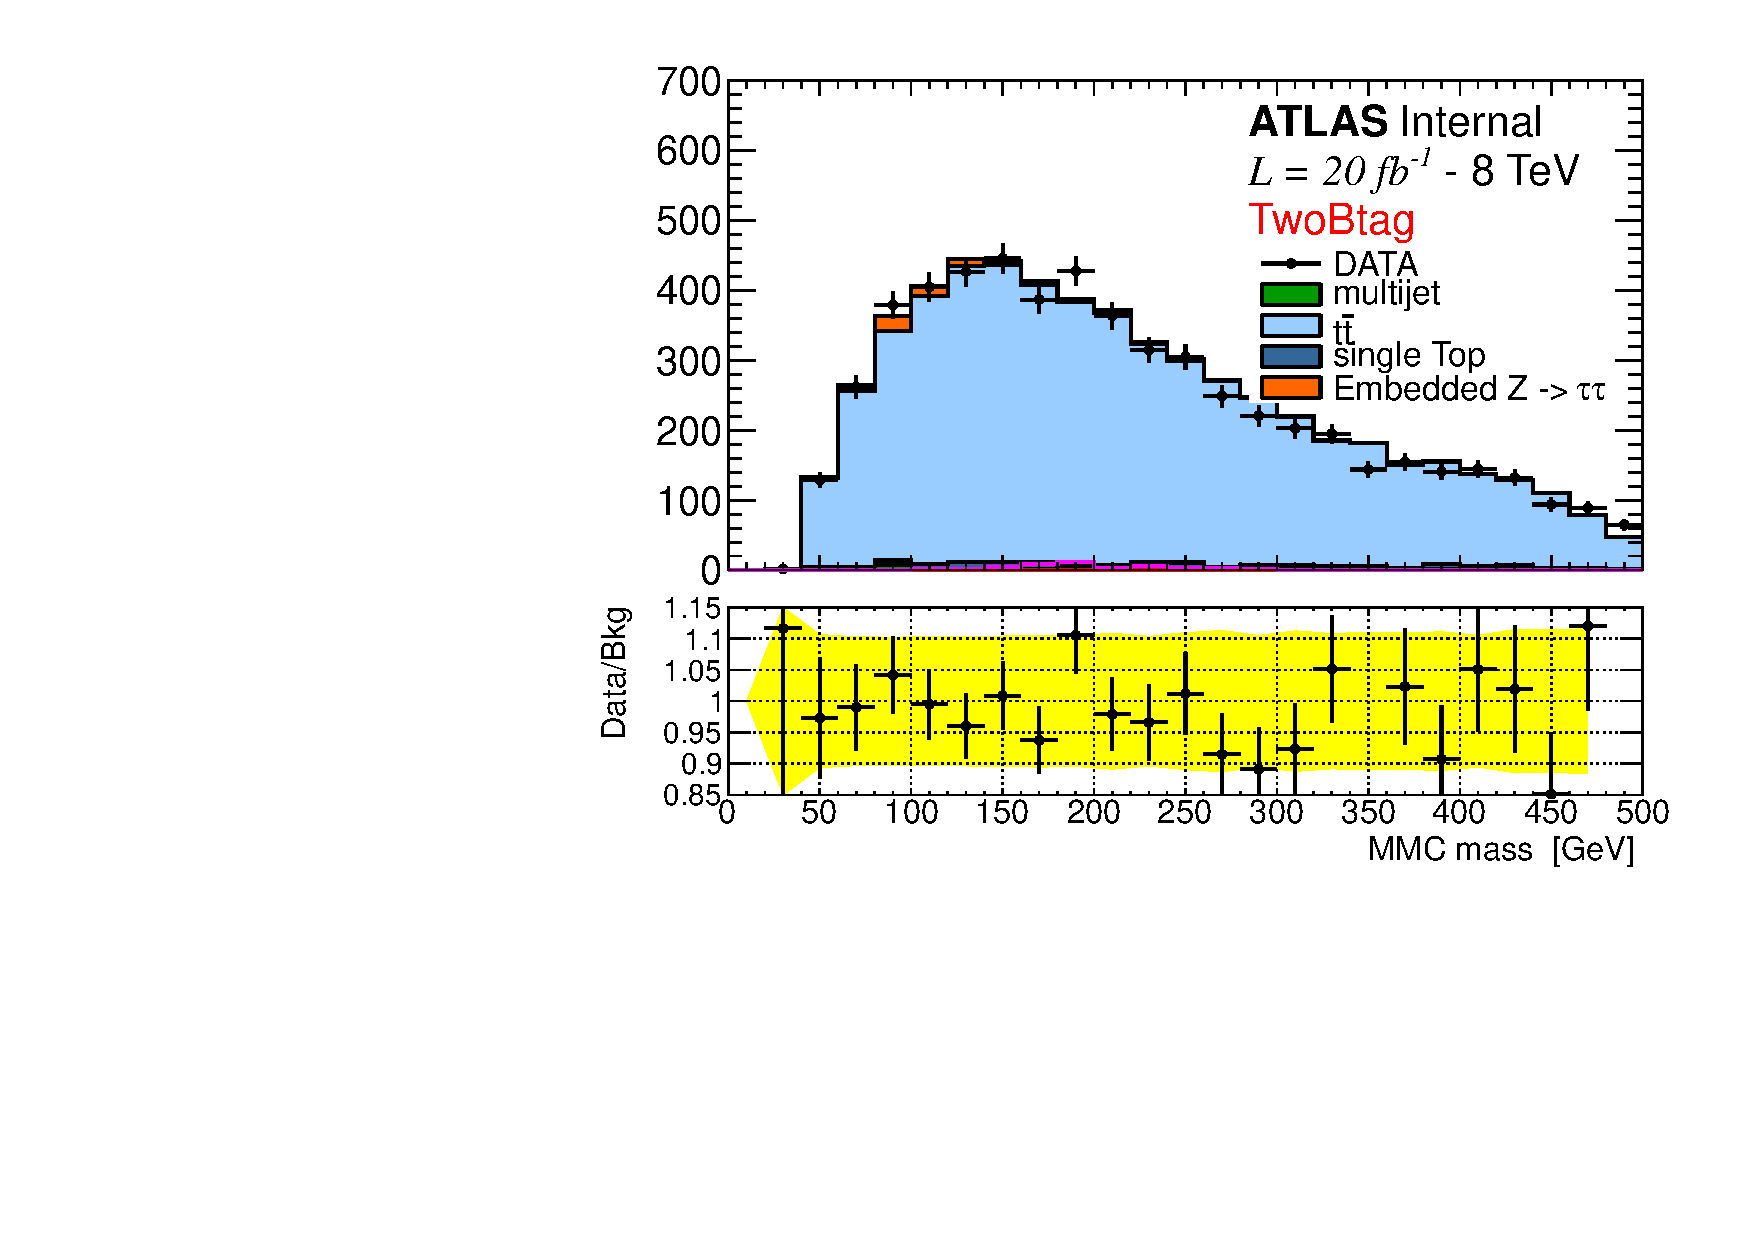
\includegraphics[page=1,width=0.45\textwidth]{figure/bg_estimation/std_plots_twoBtag.pdf}
        }
        \subfigure[]{%ele pT
           \includegraphics[page=6,width=0.45\textwidth]{figure/bg_estimation/std_plots_twoBtag.pdf}
        } 
        \subfigure[]{%Muon pt
            \includegraphics[page=8,width=0.45\textwidth]{figure/bg_estimation/std_plots_twoBtag.pdf}
        }

    \end{center}
    \caption{ Distributions  of a) the MMC mass, b) the transverse momentum of the electron $\pt(e)$ and c) the transverse momentum of the muon $\pt(\mu)$, for both data and MC in the \ttbar control region. The uncertainties on the points for the ratio plot show the statistical uncertainty on the data to background ratio, whereas the yellow band show the total systematic uncertainty on this ratio.} 
   \label{fig:kinematicsttbar}
\end{figure}


\begin{figure}[ht!]
     \begin{center}

        \subfigure[]{
            \label{fig:cuts_a} %DPhi
            \includegraphics[page=12,width=0.45\textwidth]{figure/bg_estimation/std_plots_twoBtag.pdf}
        }
        \subfigure[]{%CosDphi
            \label{fig:cuts_b}
            \includegraphics[page=13,width=0.45\textwidth]{figure/bg_estimation/std_plots_twoBtag.pdf}
        }\\
        \subfigure[]{%Ht
            \label{fig:cuts_c}
            \includegraphics[page=10,width=0.45\textwidth]{figure/bg_estimation/std_plots_twoBtag.pdf}
        }
        \subfigure[]{%Lep+Et
            \label{fig:cuts_d}
            \includegraphics[page=11,width=0.45\textwidth]{figure/bg_estimation/std_plots_twoBtag.pdf}
        }

    \end{center}
    \caption{Distributions of a) $\Delta\phi(e-\mu)$,
      b) $\sum\cos\Delta\phi$, c) \SumLtMET and d) \Ht , for both data and MC in the \ttbar control region. The uncertainty on the points for the ratio plot show the statistical uncertainty on the data to background ratio, whereas the yellow band show the total systematic uncertainty on this ratio.}
   \label{fig:cutsttbar}
\end{figure}


\subsection{Multi-jet Background}
\label{sec:qcd}

The QCD multi-jet background represents an important background, 
especially in the b-veto category, due to its high cross-section and the 
relatively low cut on lepton \pt used in this analysis. This
background is evaluated by a data-driven technique, the so-called ABCD method.
The ABCD method consists of splitting the data sample in four regions: the
 signal region (SR) and three control regions (CR), where the control
regions are mutually orthogonal and designed to be enriched in
multi-jets events. The four regions are defined by using the charge correlation
between the leptons and the isolation cuts used in the lepton preselection. 
To obtain regions rich in multi-jet background, the selections on both
the calorimetric and tracking isolation are inverted with respect to the
nominal ones described in Section~\ref{sec:eventsel}. Hence it is
possible to define four regions: opposite sign (OS) or same sign
(SS) with respectively isolated or anti-isolated leptons. Historically
the letters A-D are assigned to this regions for a quicker reference as
defined in Table~\ref{table:qcd}.

\begin{table} [ht]
\centering
\begin{tabular}{c c c }
\hline
Region & Lepton Charge & Lepton Isolation \\ [0.5ex]
\hline
A (signal region) & OS & isolated \\
B & SS & isolated \\
C & OS & anti-isolated \\
D & SS & anti-isolated \\ [1ex]
\hline
\end{tabular}
\caption{QCD background estimation control regions, defined by having leptons with opposite signs (OS) or same signs (SS) and by having the leptons either isolated or anti-isolated.}
\label{table:qcd}
\end{table}

An assumption of the ABCD method is that multi-jet backgrounds
populate the OS and SS events independently of lepton isolation
criteria and hence that the ratio of OS/SS events is uncorrelated 
with the lepton isolation selections. In this case, the number of QCD events in the signal region $A$ 
can be estimated from the yield of multijet events in the control regions $B$, $C$ and $D$, using the equation
\begin{equation} \label{eqn:qcdest}
N_{A}  = N_{B} \times \frac{N_{C}}{N_{D}} =  N_{B} \times \rqcd
\end{equation}
%Here is  assumed that the events in the control regions come solely from QCD multi-jet processes, contamination
%from electroweak (W and Z + jets, dibosons) and top processes
%($t\bar{t}$ and single top production) are  subtracted in each control region 
%using the MC prediction for their event yield.  
To obtain the multijet yields in the data CRs, the contamination
from electroweak (W+jets, Z+jets and dibosons) and top processes
($t\bar{t}$ and single top production) are  subtracted in each control region 
using the MC prediction for their event yield.  Tables~\ref{table:qcd_yield_btag}~and~\ref{table:qcd_yield_bveto}
show the event yield
% in the b-tagged and b-veto categories, respectively,
for each CR throughout the full cut-flows, along with the
predictions of non-QCD multi-jets events which are subtracted.
Signal contamination has been checked in all the three control regions for different 
mass points. For the range of $m_{A}$ and $\mathrm{tan}\beta$ considered in this analysis, the highest signal contamination 
is seen in region B for the mass point $m_{A} = 300$ GeV, where at $\mathrm{tan}\beta = 50$ a contamination 
of 0.2\% is observed. This value is mainly due to b-associated production and,
as it scales with the cross section, for $\mathrm{tan}\beta = 20$ would be an order of magnitude smaller.

Shapes of kinematic distributions for QCD events are taken from the
control region B, even though this region suffers from lower statistics than either region C or D.
This choice is made to avoid a shape bias due to the trigger:  an isolated trigger is used for electrons (as described in Section~\ref{sec:eventsel}), where the offline requirement equivalent to this trigger choice is $\ptcone20/\pt <0.1$.
Figure~\ref{fig:BvsD} shows the comparison between the electron \pt~ distributions in isolated and anti-isolated events, both for SS control regions. Here high \pt~ electrons are suppressed due to isolation requirement of the the trigger. 
Eventually the trigger isolation requirement could
bias also the ratio OS/SS - this possibility has been checked carefully
in a dedicated study and reported in Appendix \ref{appendix:qcd}.
To a good approximation, such trigger effects cancel out in the ratio
OS/SS, so no systematic is applied to the ratio because of this.

To test the ABCD method predictions an additional control region has been defined with the following selections:
\begin{itemize}
\item \MET $< 20$ GeV
\item \Ht $< 70$ GeV and \SumLtMET$ < 50$ GeV
\item $0 < \mmc < 80$ GeV  	 
\end{itemize}
%{\bf This control region is designed to enhance multi-jet background with respect to \Ztautau.}
Figure~\ref{fig:ABCD_cr} shows the \mmc distribution for this region with and without b-tagging requirements. 
Agreement between data and the background model is found in this control region within statistical and 
detector related systematics uncertainty. 

\begin{figure}[tp]
	\begin{center}
	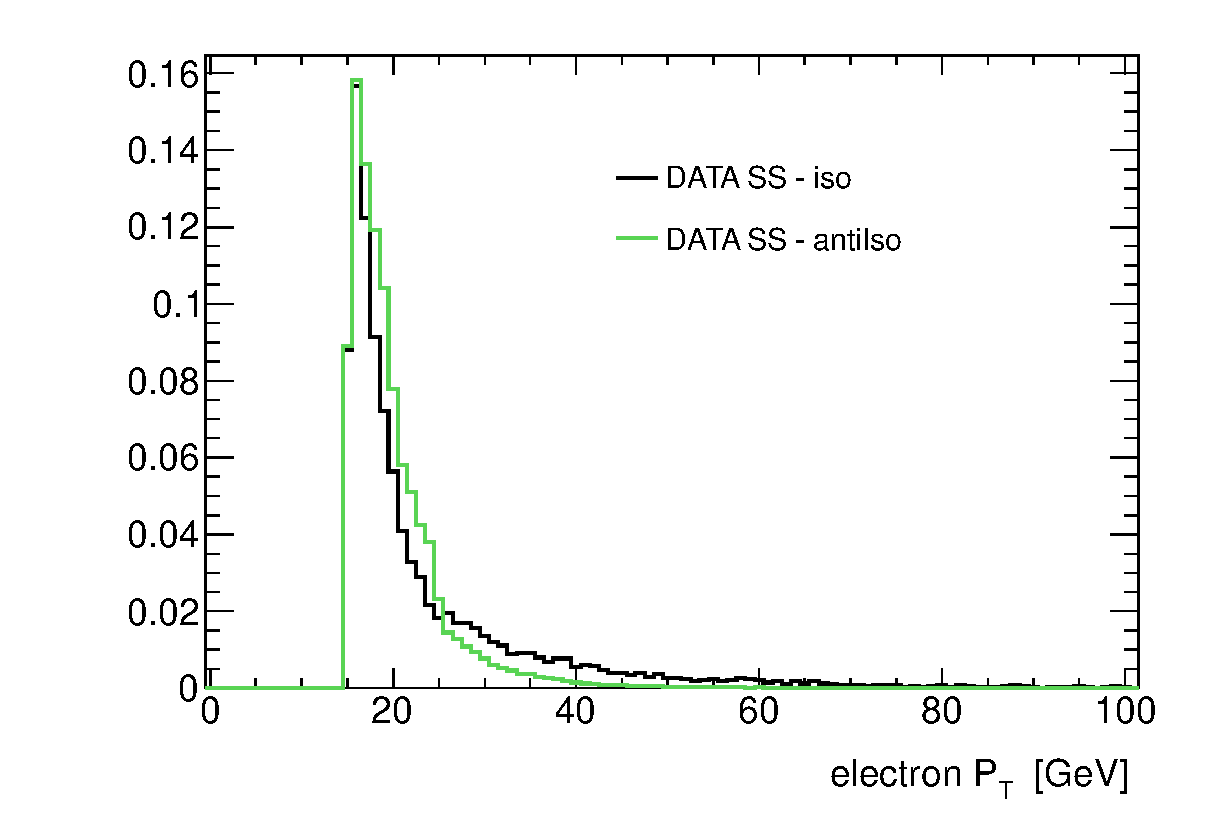
\includegraphics[width=9cm]{figure/ABCD_regionB_Vs_regionD}
	\end{center}
	\caption{Comparison of the electron \pt~distribution in region B and region D, showing the bias due to the trigger. 
	The histograms are normalised to the same area.}
	\label{fig:BvsD}
\end{figure}
%%%%	this table is not that useful

%\begin{table} [p]
%	\caption{Contribution to the different control regions from non-QCD background, after the preselection. }
%	\centering
%	\begin{tabular}{ c c c c c c c}
%%%%%%%%%%%%%%%%%%%%%%%%%%%%%%%%%%%%%%%%%%%%%%%%%%%%%%%%
%\hline
%Region  &  \Ztautau	 & $t\bar{t}$	 & W + jets	 & $Z \rightarrow ll$ + jets & Single Top 	& Dibosons \\ [0.5ex]
%\hline
%  B 	& 341 	$\pm$ 6	&	700$\pm$ 11	&	3398$\pm$ 180	& 830 $\pm$ 58	     &	178$\pm$ 8 		&   612$\pm$ 10  \\
%  C 	& 16 	$\pm$ 2	&	719$\pm$ 12	&	409$\pm$ 50	& 17 $\pm$ 4	     &	103$\pm$ 6		& 13$\pm$ 1 \\
%  D 	& 8	$\pm$ 2	&	539$\pm$ 10	&	49$\pm$	12	& 24$\pm$  7	     &	67$\pm$	 4		& 6$\pm$ 1 \\[1ex]
%\hline
%%%%%%%%%%%%%%%%%%%%%%%%%%%%%%%%%%%%%%%%%%%%%%%%%%%%%%%
%	\end{tabular}
%	\label{table:qcd_mc}
%\end{table}


%%%%%%%%%%%%%%%%%%%%%%%%%%%%%%%%%%%%%%%%%% PUT FINAL NUMBERS!!!!!!!!!!!!!!!! %%%%%%%%%%%%%%%%%%
\begin{table} [p]
	\begin{tabular}[c]{l r c c c c}
%%%%%%%%%%%%%%%%%%%%%%%%%%%%%%%%%%%%%%%%%%%%%%%%%%%%%%
\hline 
\hline 
Selection  &  		& B & C  & D &  \rqcd \\
\hline
Preselection 	&   Data	&6189			&604628			&312901		    &	1.929 $\pm$  	0.004		\\
	        &   non-QCD	&2510 $\pm$  180  	&1090 $\pm$   30  	&730	$\pm$ 35    &				\\
\hline
B-tag	     	&   Data	&419		&44619 			&27257		    &	1.64	$\pm$	0.01	\\
	     	&   non-QCD	&215 $\pm$  10	&310 $\pm$	12	&277 	$\pm$ 13    &				\\
\hline
$\Delta\phi(e-\mu)$  &   Data		&230		&38810 			&23316		    &	1.67	$\pm$	0.01	\\
	     &   non-QCD	&104 $\pm$ 6	&200 $\pm$	10	&175	$\pm$ 7	    &				\\
\hline
$\sum\cos\Delta\phi$ &   Data & 149		&31379 			&18779		    &	1.67	$\pm$	0.02	\\
	     &   non-QCD      & 67 $\pm$ 5	&127 $\pm$	8	&114 $\pm$	6   &				\\
\hline
$\sum H_T$ &   Data	      & 83		& 27781 		&15626		    &	1.78	$\pm$	0.02	\\
	&   non-QCD	      & 23 $\pm$  4	& 25 $\pm$	3	& 22 $\pm$   3	    &				\\ 
\hline
\SumLtMET &   Data	&71		&27735 	&15590		    &	1.78	$\pm$	0.02	\\
	     &   non-QCD	 & 10 $\pm$	3	& 22  $\pm$ 3		&18	$\pm$ 2	    &			\\
\hline
$\mmc > 0.$    &  Data	& 70	& 27634 	& 15522		    			    &	1.78	$\pm$	0.02	\\
	     &   non-QCD	& 9 $\pm$ 3	& 20  $\pm$ 3		&17	$\pm$ 2	    &			\\[1ex]
\hline
\hline
%%%%%%%%%%%%%%%%%%%%%%%%%%%%%%%%%%%%%%%%%%%%%%%%%%%%%%
	\end{tabular}
	  \caption{QCD background estimation as a function of the analysis selections for the b-tagged category. The yields for the different control regions, as well as the scaling factor \rqcd, are reported. The error on the \rqcd is statistical only.}
	\centering
	\label{table:qcd_yield_btag}
\end{table}


\begin{table} [p]
	\begin{tabular}[c]{l r c c c c}
%%%%%%%%%%%%%%%%%%%%%%%%%%%%%%%%%%%%%%%%%%%%%%%%%%%%%%%
\hline
\hline 
Selection  &  		& B & C & D &  \rqcd \\ 
\hline
Preselection 	&   Data	&6189			&604628			&312901		    &	1.929 $\pm$  	0.004		\\
	        &   non-QCD	&2510 $\pm$  180  	&1090 $\pm$   30  	&730	$\pm$ 35    &				\\
\hline
B-veto	     	&   Data	&5673		  & 558217 		& 284847		    &	1.960	$\pm$	0.004	\\
	     	&   non-QCD	&2220	$\pm$ 180 & 710 $\pm$ 30	& 415 $\pm$	30	    &				\\
\hline
$\Delta\phi(e-\mu)i$  &   Data		&4610		&532583 		&271404		    	    &	1.962	$\pm$	0.005	\\
	     &   non-QCD	&1700 $\pm$170	&580 $\pm$	30	& 345 $\pm$	30	    &				\\
\hline
$\sum\cos\Delta\phi$ &   Data& 3417	&486747 		& 247712	   		    &	1.965	$\pm$	0.005 	\\
	     &   non-QCD     & 1120  $\pm$ 100	& 370 $\pm$ 	20		& 230 $\pm$	20  &				\\
\hline
$\mmc > 0.$    &  Data		& 3177		& 479967 		& 244276	    	    &	1.965	$\pm$	0.005	\\
	     &   non-QCD	& 1000 $\pm$ 100	& 300  $\pm$ 17		&190	$\pm$ 20    &			\\[1ex]
\hline
\hline
%%%%%%%%%%%%%%%%%%%%%%%%%%%%%%%%%%%%%%%%%%%%%%%%%%%%%%%
	\end{tabular}
	\caption{QCD background estimation as a function of the analysis selections for b-veto category. The yields for the different control regions, as well as the scaling factor \rqcd, are reported. The error on the \rqcd is statistical only.}
	\centering
	\label{table:qcd_yield_bveto}
\end{table}



\begin{figure}[tp]
	\begin{center}
	     
	\subfigure[]{
		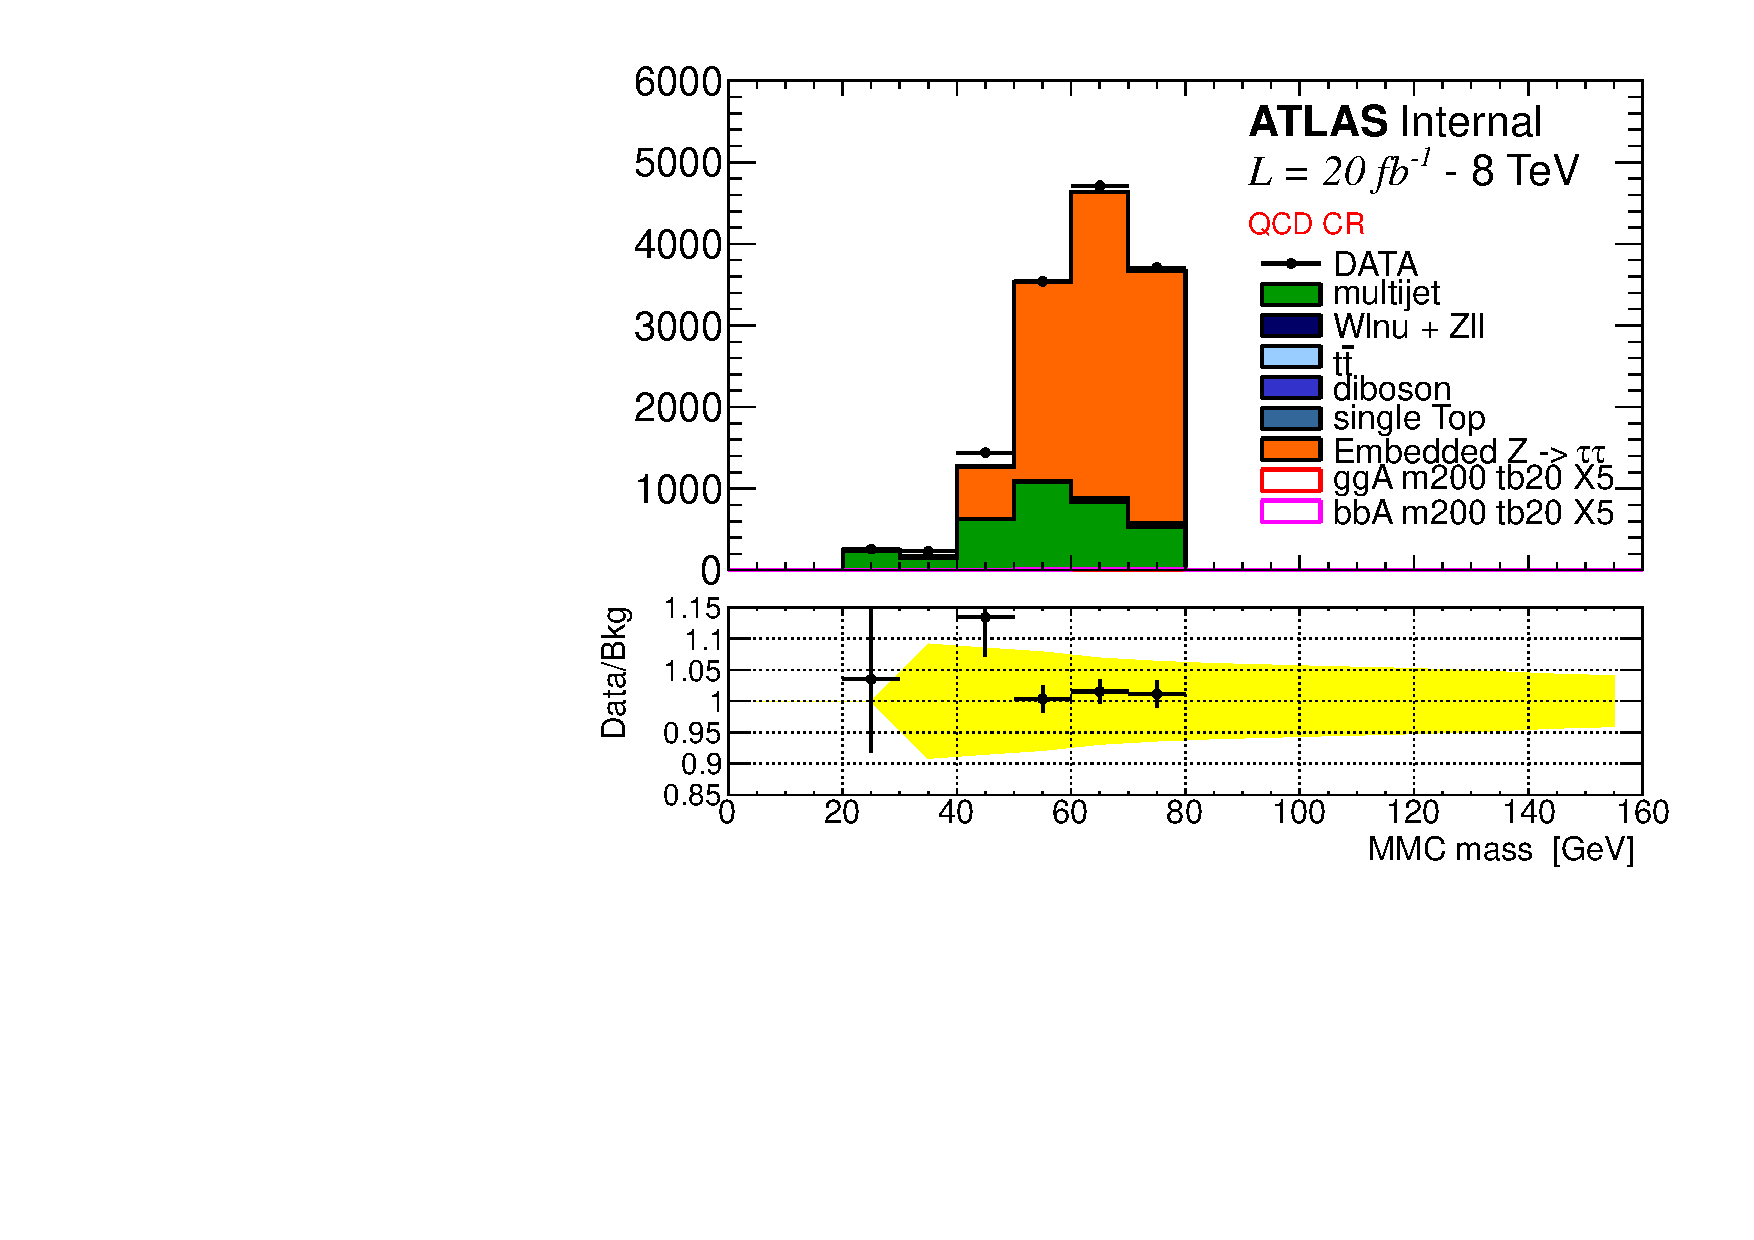
\includegraphics[page=1,width=0.49\textwidth]{figure/QCD/qcd_CR_emb.pdf}
	        }
	\subfigure[]{
  	\includegraphics[page=5, width=0.49\textwidth]{figure/QCD/qcd_CR_emb.pdf}
	}
	
	\end{center}
	\caption{\mmc distribution for QCD cross check regions defined in section \ref{sec:qcd} (a) and for the same CR when in addition one b-tagged jet is required (b). }
	\label{fig:ABCD_cr}
\end{figure}


Systematic uncertainties are assigned on the scaling factor \rqcd and on the shape of
the discriminating variable \mmc to take into account any correlation between isolation and charge 
of the leptons, details on the systematic uncertainty evaluation are addressed in Section~\ref{sec:Systematics}.

\subsection{$Z \rightarrow \tau\tau$ + Jets Background}
A good understanding of the background from \Ztautau decays is vital to this
analysis. Unfortunately, for a light Higgs boson, it is impossible to completely separate \Ztautau decays 
from the signal - hence a signal free data control region cannot be defined.
However, thanks to the small Higgs coupling to muons, \Zmumu decays provide a good starting point to 
model \Ztautau events in a data-driven way. Hence a hybrid Data-MC sample, known as "Embedding" is used to model the \Ztautau background: 
$\Zmumu$ candidates are selected in data, then the two muons from the $Z$ decay are substituted with the decay 
products from simulated taus, those taus have the same kinematics as the original muons. 
Further details may be found in \cite{Embedding, SMold}.

%The selection of the \Zmumu input data requires exactly two combined, opposite charged
%muons, where the leading muon has a transverse momentum $\pt > 20 \GeV$ and 
%the subleading muon $\pt > 15\GeV$. Both muons are requited to lie within $|\eta|<2.5$ and to be isolated with 
%$\ptcone 20/\pt<0.2$ (see Section~\ref{sec:presel}). Additionally 
%the invariant mass of the two muons is required to be in the range $M_{\mu\mu} > 40$ GeV.
%Once the muon pair events are selected, all tracks and calorimeter cells associated to the muons are 
%removed from the \Zmumu data event. Finally, the calorimeter cell energy and tracks from the simulated tau decays
%are added to the data event and the event is re-reconstructed.

%A set of corrections are applied to correct for the muon trigger efficiency, the muon reconstruction efficiency and other additional effects
%related to the original \Zmumu events. Finally, as the trigger is not emulated in the embedding sample, 
%an additional correction is applied to emulate the electron and muon trigger efficiencies in the final \Ztautau embedded events. 
%For a full description of the corrections and validation see \cite{SMnew}.

The Embedding technique, which uses \Zmumu decays to 
model \Ztautau events in a data-driven way, is described in Section~\ref{sec:data_mc}. 
As there is no simulation of the trigger in the embedding samples, the event yield
is normalised to ALPGEN \Ztautau at preselection stage. Furthermore a set of corrections, as described in \cite{SMnew}, are
applied to account for the trigger and muon reconstruction efficiency in the original \Zmumu events, to emulate the trigger efficiency in the embedded \Ztautau events and to correct for the b-layer requirements that are not modelled in the embedded events.

The Embedding technique has been validated in several studies, detailed in~\cite{Embedding, SMnew}, which show a good description of 
data and \Ztautau MC by \Ztautau events from Embedding. In the context of this analysis, figures~\ref{fig:emb_vs_alp1} and \ref{fig:emb_vs_alp} show comparisons of various kinematic variables between
data, embedding and ALPGEN \Ztautau events at preselection. No significant deviation is seen between the \mmc distribution of the embedding and ALPGEN samples (here the data \mmc distribution is not shown). However other relevant variables for this analysis, such as the \MET and the number of b-jets, are slightly better described by embedding. Additional plots are reported in appendix~\ref{appendix:additionalEmb}.

\begin{figure}[tp]
     \begin{center}

            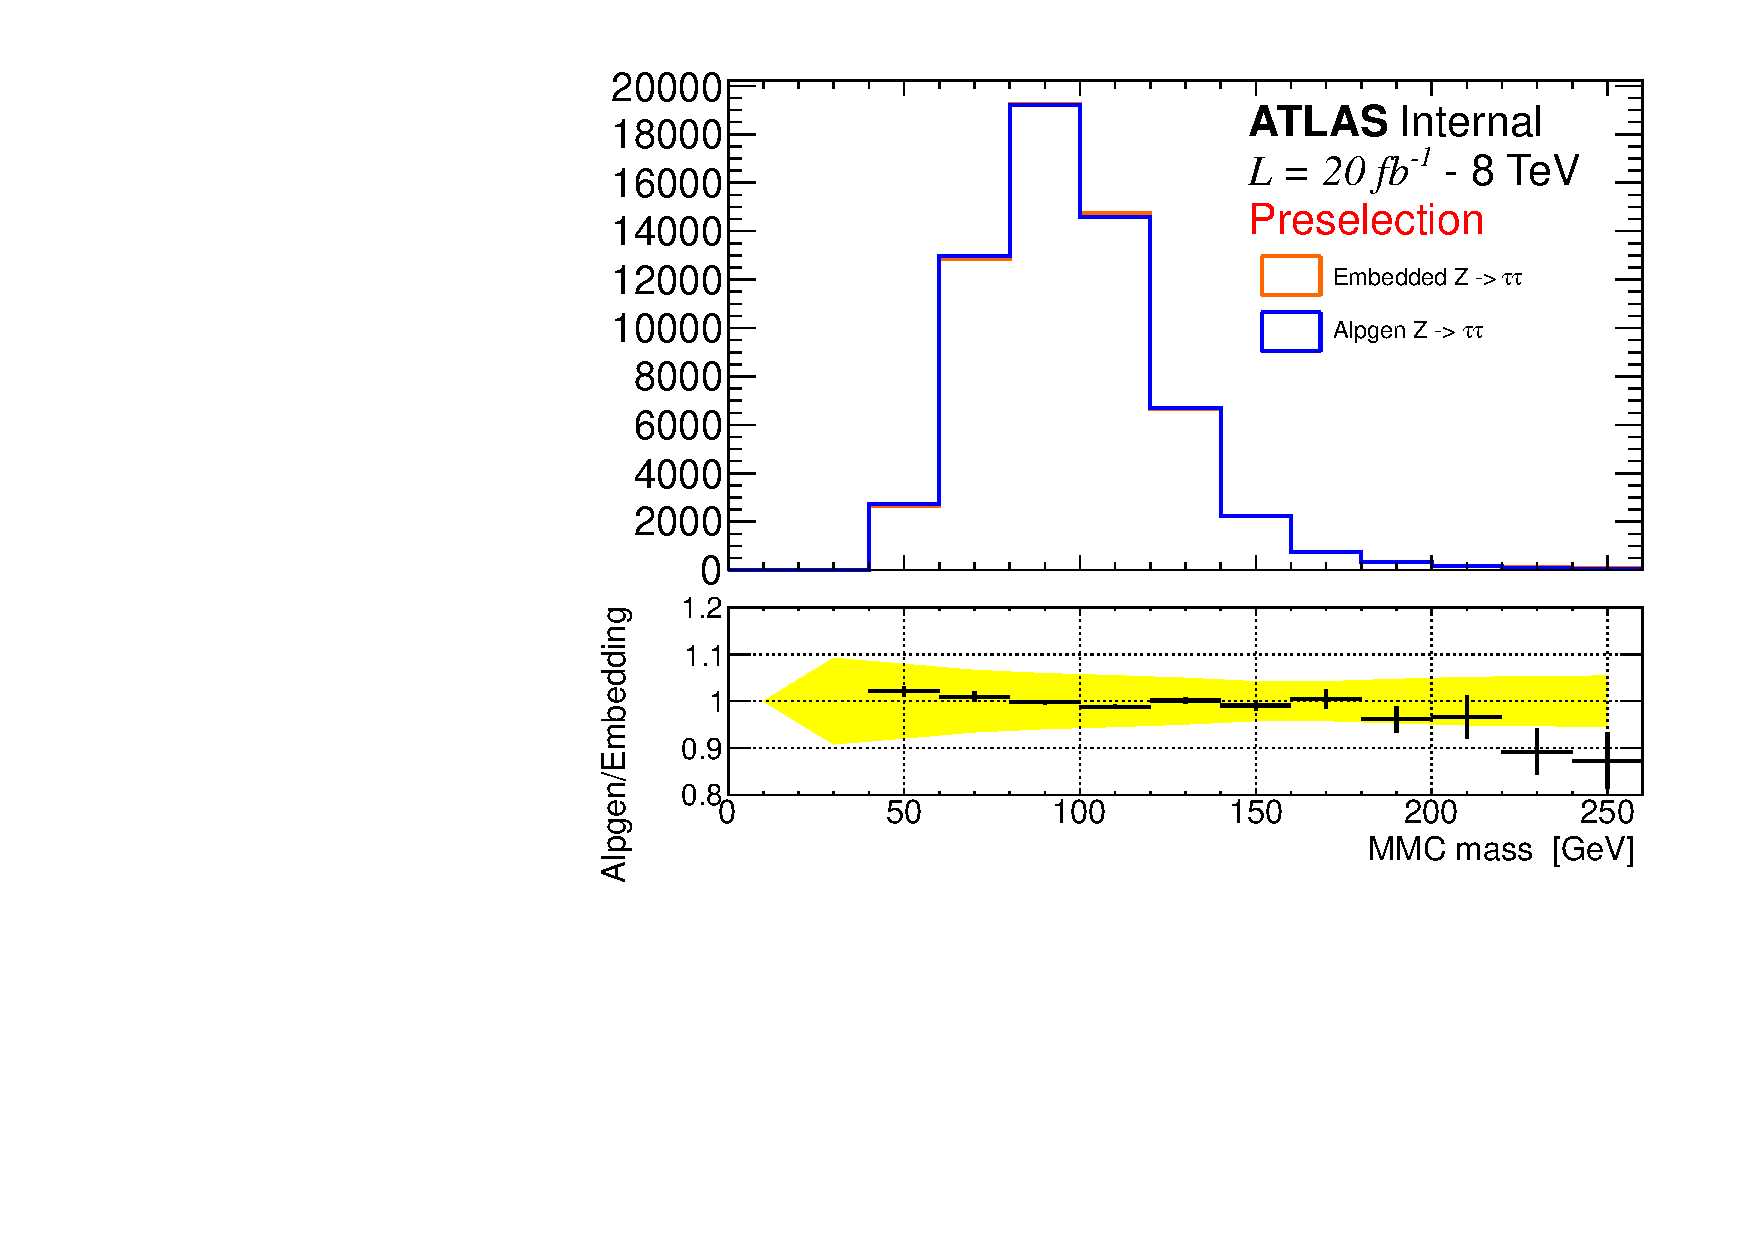
\includegraphics[page=1, width=0.6\textwidth]{figure/bg_estimation/std_plots_emb.pdf}
\end{center}
    \caption{Comparison between the embedded \Ztautau and ALPGEN for $\mmc$ distributions.}
   \label{fig:emb_vs_alp1}
\end{figure}


\begin{figure}[tp]
     \begin{center}

           \includegraphics[page=2, width=0.6\textwidth]{figure/bg_estimation/std_plots_emb.pdf}
            \includegraphics[page=3, width=0.6\textwidth]{figure/bg_estimation/std_plots_emb.pdf}

    \end{center}
    \caption{Comparison between embedded \Ztautau and ALPGEN for $\MET$ and the number of b-tagged jets distributions.
	Data are superimposed, with the contribution of non-\Ztautau are subtracted.}
   \label{fig:emb_vs_alp}
\end{figure}


%plot comparing embedding and ALPGEN Et miss and b-tagging, data -MC not Ztautau and compare data alp and emb.

As the embedding sample is based on selecting \Zmumu candidates in data, the selections assure a rather 
pure \Zmumu sample. However further selections used in this analysis, for example the b-tagging requirements, 
could enhance the contamination fraction from other processes in the embedding sample. Hence dedicated studies have been
made to estimate the $t\bar{t}$ and QCD multi-jet contamination in the embedding sample.
The \ttbar~ contamination is estimated by evaluating the embedding sample yield in a two b-tag control region,
as described in Section~\ref{sec:top_est}. These events are assumed to be solely from $t\bar{t}$
and their yield in the signal region is extrapolated using POWHEG-PYTHIA $t\bar{t}$ simulation sample.
Table~\ref{table:emb_cont_tt} shows a summary for the top contamination in embedding and this contamination is hence taken to be negligible. The multi-jet contamination can be estimated starting 
from the embedding yield of opposite sign anti-isolated events (region C).
%one should not use SS regions because embedding already requires leptons to be OS, then would be biased
Assuming all events in this CR as QCD multi-jet events, the contamination in the SR 
can be estimated using the ABCD method (see Section\ref{sec:qcd}). The \rqcd factor 
used in this case is evaluated using a mu-mu final state CR with the same kinematics selections
used in the definition of the embedding sample. Table~\ref{table:emb_cont_qcd}
shows the estimated contamination of QCD multi-jet in embedding. 
We  consider contamination effects negligible.

\begin{table} [p]
\centering
\begin{tabular}{c c c c c}
\hline
\hline
 & Embedding yield in CR & Transfer factor & Estimated events in SR & Contamination \\ [0.5ex]
\hline
b-tag & $84 \pm 9$  & $(2.6 \pm 0.1) \times 10^{-2}$ &  $2.2 \pm 0.2$&  0.5 \% \\
b-veto & $84 \pm 9$ & $(1.74 \pm 0.02) \times 10^{-1}$ & $15 \pm 2$ & 0.03 \% \\[1ex]
\hline
\end{tabular}
\caption{Evaluating embedding $t\bar{t}$ contamination using a two b-tag CR. The transfer factor is the
multiplicative factor that allows to estimate events in SR from the CR. }
\label{table:emb_cont_tt}
\end{table}

\begin{table} [tp]
\centering
\begin{tabular}{c c c c c}
\hline
\hline
 & Embedding yield in CR & Transfer factor & Estimated events in SR & Contamination \\ [0.5ex]
\hline
B-tag  & $12 \pm 3$ & $ (7 \pm 1) \times 10^{-3}$ &  $(8.4 \pm 0.3) \times 10^{-2}$ &  0.03 \% \\
B-veto & $390 \pm 20$ & $(2.5 \pm 0.1) \times 10^{-2}$ & $10.0 \pm 0.5$ & 0.02 \% \\[1ex]
\hline
\end{tabular}
\caption{Evaluating embedding contamination due to QCD multi-jet using ABCD method, 
the CR here is with OS anti-isolated events (region C). The transfer factor is the
multiplicative factor that allows to estimate events in SR from the CR, in this case is $N_{B} / N_{D}$
and is evaluated using mu-mu final state with the same kinematic selection used in the 
definition of the embedding sample. }
\label{table:emb_cont_qcd}
\end{table}


\section{Systematic Uncertainties}
\label{sec:Systematics}

This section describes the range of systematic uncertainties
that are relevant for this analysis. To account for differences in the detector responses between simulation and data a 
set of corrections are applied either at object reconstruction level, as described in section~\ref{sec:presel}, or at the event level. 
The uncertainties on such corrections are considered as detector-related systematic uncertainties and are detailed in section~\ref{sec:sys:sys_det}. Further systematic uncertainties related to data-driven methods for backgrounds estimation
are described in section~\ref{sec:sys_bg}.  For
samples which rely on MC simulation, theory-related
systematics, which include uncertainties on the cross-section and
uncertainties on the acceptance of analysis selections,  
are finally described in section~\ref{sec:sys_theory}.

Each single systematic can contribute separately to the uncertainty on the
final event yield and on the shape of the $\mmc$
distribution that is used as the discriminating variable for the limit derivation. These shape systematics are
documented in appendix~\ref{appendix:shapeNPs}. Systematic uncertainties that do not effect the
mass shape distribution and have an impact on the event yield of a samples of less than 0.5\% are 
neglected in the final limit calculations.
%hey infact do not have any significant effect on the final expected limits.


\subsection{Detector-related Systematics Uncertainties}
\label{sec:sys:sys_det}

%Here we address systematic uncertainty related to object reconstruction and event 
%corrections, those correction are based on the measure of some relevant parameter, each of those parameter correspond 
%to a "nuissance paremeter" in our probability model as described in Section~\ref{sec:ExclusionLimits}.
%
%Reciepe:
%
%Correction are measured elsewhere, those correspond to property of the object like 
%energy scale or resolution, or are related to event properties like pieleup ecc.., along with theyr mean value
%an uncertainty is evaluated,
%We variate each parameter independently (one sigma up or down) according with their uncertainty and evaluate the impact on the analysis yield for each sample. An intepolation algorithm then defines what is the impact of that nuissance parameter
%on the analysis for any value. In the following we describe in detail the uncertainties on each used correction,
%table~\ref{tab:ExpSys:btag} and~\ref{tab:ExpSys:bveto} briefly summarize the impact on the samples yield for the most significant systematic uncertainty considered. 



\paragraph{Luminosity}
The uncertainty on the integrated luminosity is taken to be 2.8\% \cite{luminosity}.

\paragraph{Pileup}
As described in Section~\ref{sec:SimSamples}, MC events are re-weighted according to reproduce the average interactions per bunch crossing, $<\mu>$, seen in data. It has been seen
that a proper description of the minimum bias vertex multiplicity is obtained if the $<\mu>$ 
value in MC is first scaled by a factor of $1.11 \pm 0.03$ before re-weighting to match data. The uncertainty
on this value is taken as a systematic uncertainty for the analysis.

\paragraph{Trigger Efficiency}
The scale factors used to correct for the differences in trigger efficiency between data and MC for the triggers considered in this analysis are described in Section~\ref{sec:presel:TriggerCorr}. The uncertainties on these scale factors are used to estimate the systematic uncertainty due to the understanding of the trigger efficiencies. 
Systematic uncertainties on both the single electron and
electron-muon trigger efficiency are considered independently, by varying the scale factors coherently by their uncertainties.
The uncertainties are aproximately 1-2\%, depending on the $\pt$ and $\eta$ of the leptons.

In the embedding sample, the trigger is emulated by applying weights to the event
topology. In addition, corrections are applied to correct for trigger efficiency in the original $\Zmumu$ events. 
These corrections are likewise varied coherently by their uncertainties to estimate the trigger systematic uncertainty 
for this background. Hence, the trigger systematic uncertainty for embedding is considered independently
from that for the other backgrounds.

\paragraph{Electrons}
Two types of uncertainty on reconstructed electron objects are considered:
the first are related to electron identification and reconstruction efficiencies, respectively. 
The second type are related to electron energy scale and resolution corrections.
The effect of the uncertainties on the reconstruction and identification is estimated by coherently varying the applied scale factors by their 
associated uncertainties. The effect on the final yield of each sample from both of the uncertainties is then 
summed in quadrature to give the overall uncertainty (referred to as "Electron SF").
The energy scale uncertainties are split into a set due to six different nuisance parameters \cite{EGammaEnergy}. 
However many of them are found to have a negligible effect on the overall yield. Only the uncertainties 
related to the $Z \rightarrow ee$ measurement ("Electron Zee") 
and due to low momentum electrons ("Electron LOWPT") are found to give a significant effect. Both of these two uncertainties affect the mmc mass distribution, in particular for 
\Ztautau samples, hence these are considered as shape systematics in the limit calculation.
We sum in quadrature all the other uncertainties related to energy scale and resolution (referred as "Electron E.").
%PUT IN APPENDIX OR HERE PLOTS OF SHAPE

\paragraph{Muons}
The uncertainty on muon identification efficiency depends on the charge and momentum of the muon.
Typically these uncertainties are of the order of a fraction of percent, and are referred as "Muon ID". 
The uncertainties on the muon momentum are considered by smearing  the inner detector and muon spectrometer \pt~ 
values and changing the \pt~ scale within their uncertainties. 
Each component is varied individually and the individual variations in event yields 
summed in quadrature. The total systematic uncertainty is referred to here as "Muon E.".

\paragraph{Taus}
Hadronic tau object are only used in the analysis as a veto. Uncertainties on both tau energy scale 
and identification efficiency have been investigated and are found to be negligible for this analysis.

\paragraph{Jets}
The systematic uncertainties on the Jet Energy Scale (JES) are split up into multiple sets of nuisance parameters, which
 hence contain a full treatment of the bin-by-bin correlations of the uncertainties. The overall uncertainty on the JES ranges 
 between 3\% and 7\%, depending on the $\pt$ and $\eta$ of the jet. The recommendation \cite{TWIKI_JETMET} to propagate each individual 
 source of uncertainty through the full analysis is followed. In this analysis the reduced set of fourteen uncertainties, know as 
 \verb=InsituJES2012_14NP=, have been considered: these include two uncertainties for eta intercalibration, four pile-up 
 uncertainties, a high-$\pt$ uncertainty and an uncertainty for MC non-closure. Of these, only the terms "JES Effective 1", 
 "JES Effective 2" and "JES Effective 3", the pileup uncertainty as a function of the number of primary vertices ("JES Pileup-NPV") and the uncertainty due to the jet area ("JES Pileup-Rho") have a significant effect on the event yields. Additionally, 
 the uncertainty related to the fraction of quark to gluon jets ("JES Flav. Comp") and on the different response to them ("JES Flav. Resp.") are considered. The additional uncertainty assigned to the b-jet energy scale, referred as "JES B", is also 
 significant to this analysis. Uncertainties related to theory and modelling ("JES EtaModelling") also contribute to this 
 analysis. Finally the effect of the jet energy resolution ("JES Resolution") is evaluated applying a smearing to the jets, the 
 resulting effect on the yield is symmetrised.

\paragraph{b-Tagging}
Uncertainties on the knowledge of both the b-tag and mistag efficiencies for the 70\% working point of the MV1 b-tagger are
 considered in this analysis. Hence both the b-tag and b-veto channels are affected. The tag and mistag efficiencies are
  considered to be totally anti-correlated. Uncertainties for b-quark, c-quark and light or gluon initiated jets, referred to as 
  "B  Eff.", "C Eff." and "L Eff." respectively, are considered. In the rare case where a hadronically decaying 
  tau is b-tagged, the uncertainty for c-quark induced jets is used.


\paragraph{Missing Transverse Energy}
In addition to propagating the effect of the energy scale
uncertainties for all the physics objects to the \met, the effect of
uncertainties on the ``soft-terms'' of the \met are
considered. Uncertainties on both the scale and resolution of the
soft-terms are independently propagated through the analysis and are
added in quadrature, this final term is referred as "MET" uncertainty.


\paragraph{Summary} A summary of the effect of the experimental and theoretical systematic uncertainties on signal and background yields for the b-tag and b-veto channels are shown in Table~\ref{tab:ExpSys:btag} and Table~\ref{tab:ExpSys:bveto}, respectively. It should 
be noted that the gluon fusion  signal sample suffers of poor statistics in the b-tag category. 
Hence, some of the yield differences reported are statistically dominated for these samples.
%	As a solution the mean value between all the sample mass point can be taken as measure of the single systematic, 
However the gluon fusion production mode has a negligible contribution in b-tag category.
	
\begin{table}[hp]
  \centering
  \begin{tabular}{lccccc}
    \hline\hline
      	      		   \multicolumn{6}{c}{ b-tag category uncertainties (\%)}  \\
     \hline
      Source             & Signal bbH & Signal ggH & \Ztautau &  Top 	& Other	 \\
    \hline
Electron SF  		 &2.3		   &2.0		     &	2.8    &	1.8	&2.0	 \\
Electron E.	  	 &0.7		   &1.2		     &0.5	     &0.5	&0.9	 \\
Electron LOWPT	  	 &0.4		   &0.0		     &0.4	     &0.1	&0.4	 \\ 
Electron Zee	  	 &0.3		   &0.6		     &0.4	     &0.6	&0.5	 \\
Muon ID 		 &0.3		   &	0.3	     &	0.3	     &	0.3	&0.3	 \\
Muon E.		  	 &0.5		   &7.7		     &0.1	     &0.1	&0.2	 \\
Trigger Single	Ele.  	 &0.7		   &0.5		     &0.5	     &0.8	&0.8	 \\
Trigger Dilepton	  	 &1.0		   &1.2		     &1.4	     &0.6	&0.6	 \\
Embedding MFS	  	 &-		   &-		     &0.0	     &-		&-	 \\
Embedding Iso.	  	 &-		   &-		     &1.3	     &-		&-	 \\
JES Effective-1   	 &0.5		   &0.0		     &-		     &3.8	&2.3	 \\
JES Effective-2   	 &0.6		   &7.8 	     &-		     &5.5	&2.5	 \\
JES Effective-3   	 &0.5		   &0.0		     &-		     &2.2	&2.0	 \\
JES EtaModelling    	 &1.1		   &0.0		     &-		     &4.0	&2.1	 \\
JES Pileup-NPV	  	 &0.5		   &0.0		     &-		     &1.2	&0.3	 \\
JES Pileup-Rho	  	 &0.8		   &7.8 	     &-		     &2.8	&2.2	 \\
JES FlavComp.	  	 &1.2		   &6.3		     &-		     &2.1	&4.5	 \\
JES FlavResp.	  	 &1.3		   &0.0		     &-		     &1.4	&1.9	 \\
JES BJet	  	 &1.2		   &0.0		     &-		     &4.2	&1.2	 \\
JER		  	 &1.4		   &6.3		     &-		     &2.9	&3.0	 \\	%Should be added in Framework	
B Eff		  	 &10.2		   &5.3		     &-		     &2.6	&5.0	 \\
C Eff		  	 &0.2		   &2.8		     &-		     &0.0	&1.2	 \\
L Eff		  	 &0.4		   &8.0		     &-		     &0.1	&1.2	 \\
Pileup			 &0.4		   &0.7		     &0.4	     &0.4	&0.9	 \\		%Should be added in Framework	
MET 		  	 &0.7		   &11.0 	     &0.2	     &1.0	&1.2	 \\
Acceptance		 &		   &		     &		     &		&	  \\
Cross Section	  	 &-		   &-		     &5.0	     &5.5	&7.1	 \\
Luminosity	  	 &2.8 		   &2.8	 	     &2.8 	     &2.8 	&2.8 	 \\

    \hline
    \hline
  \end{tabular}
  \caption{Summary of the effect of the experimental and theoretical systematic uncertainties on the yields of the different
	%samples used  in the b-tag channel. Here "Other" refers to the sum of all the remaining samples: $\Wln$, 
	%diboson, $\Zll$ and single top. The signal samples listed here are b-associated production and gluon 
	fusion with $m_{A}=120$ GeV and $\tan\beta=20$. 
	 Systematic uncertainties with a negligible effect are are listed with a value of 0.0
	 and those that lead to a  shape uncertainty are noted with the symbol (\textbf{s}). 
	Note that the same naming convention is respected for the actual nuisance parameters in the limit framework.}

  \label{tab:ExpSys:btag}
\end{table}


\begin{table}
  \centering
  \begin{tabular}{lccccc}
    \hline\hline
      	      		   \multicolumn{6}{c}{ b-veto category uncertainties (\%)}  \\
     \hline
      Source             & Signal bbH & Signal ggH & \Ztautau &  Top 	& Other	 \\
    \hline
Electron SF  		 &2.4		   &2.3		     &2.9 (\bf{s})	     &1.4	&1.6	 \\
Electron E.	  	 &0.4		   &0.5		     &0.4	     &0.5	&0.9	 \\
Electron LOWPT	  	 &0.3		   &0.5		     &0.4 (\bf{s})	     &0.0	&1.2  \\ 
Electron Zee	  	 &0.4		   &0.4		     &0.4 (\bf{s})	     &0.1	&0.3	 \\
Muon ID 		 &0.3		   &0.3		     &0.3	     &0.3	&0.3	 \\
Muon E.		  	 &0.1		   &0.1		     &0.1	     &0.5	&0.5	 \\
Trigger Single	Lep.  	 &0.6		   &0.6		     &0.5	     &0.9	&0.9	 \\
Trigger Dilep.	  	 &1.0		   &1.0		     &1.3	     &0.2	&0.3	 \\
Embedding MFS	  	 &-		   &-		     &0.1 (\bf{s})	     &-		&-	 \\
Embedding Iso.	  	 &-		   &-		     &0.0 (\bf{s})	     &-		&-	 \\
JES Effective-1   	 &0.2		   &0.2		     &-		     &0.4	&0.4	 \\
JES Effective-2   	 &0.2		   &0.3		     &-		     &0.3	&0.5	 \\
JES Effective-3   	 &0.2		   &0.2		     &-		     &0.2	&0.3	 \\
JES EtaModelling    	 &0.1		   &0.1		     &-		     &0.1	&0.3	 \\
JES Pileup-NPV	  	 &0.3		   &0.1		     &-		     &0.1	&0.3	 \\
JES Pileup-Rho	  	 &0.3		   &0.2		     &-		     &0.5	&0.5	 \\
JES FlavComp.	  	 &0.1		   &0.2		     &-		     &0.2	&0.5	 \\
JES FlavResp.	  	 &0.2		   &0.4		     &-		     &0.3	&0.6	 \\
JES BJet	  	 &0.2		   &0.0		     &-		     &0.5	&0.1	 \\
JER		  	 &0.5		   &0.3		     &-		     &0.6	&0.3	 \\	%Should be added in Framework	
B Eff		  	 &1.8		   &0.0		     &-		     &12.0	&0.8	 \\
C Eff	  		 &0.0		   &0.1		     &-		     &0.1	&0.0	 \\
L Eff	  		 &0.0		   &0.1		     &-		     &0.2 	&0.1	 \\
Pileup			 &0.5		   &0.8		     &0.4	     &0.3	&0.3	 \\	%Should be added in Framework	
MET  		  	 &0.2		   &0.8 	     &0.1	     &0.2	&0.5	 \\
Acceptance		 &		   &		     &		     &		&	  \\
Cross Section	  	 &-		   &-		     &5.0	     &5.5	&5.9	 \\
Luminosity	  	 &2.8 		   &2.8	 	     &2.8 	     &2.8 	&2.8 	 \\

    \hline
    \hline
  \end{tabular}
  \caption{Summary of the effect of the experimental and theoretical systematic uncertainties on the yields of the different
	samples used  in the b-veto channel. Here "Other" refers to the sum of all the remaining samples: 
	$\Wlnu$, diboson, $\Zll$ and single top. The signal samples listed here are b-associated production 
	and gluon fusion with $m_{A}=120$ GeV and $\tan\beta=20$. 
	 Systematic uncertainties with a negligible effect are are listed with a value of 0.0
	 and those that lead to a  shape uncertainty are noted with the symbol (\textbf{s}). 
	Note that the same naming convention is respected for the actual nuisance parameters in the limit framework.}
 \label{tab:ExpSys:bveto}
\end{table}


\subsection{Systematics for Data-Driven Background Estimation Methods} 
\label{sec:sys_bg}

\subsubsection{\Ztautau Embedding Systematics}
An important element of the embedding method is the subtraction of the 
calorimeter cells associated with the muons in the original \Zmumu event and their substitution with those from the simulated tau
decays. To make a conservative estimate of the systematic uncertainty on this procedure, the energy of the subtracted cells is scaled up or down by 30\%. The analysis is repeated with those modified samples and the relative uncertainty is referred as EMB\_MFS. The effect of this uncertainty on the \mmc distribution is shown in figure~\ref{fig:EmbeddingShapeNPs}. Hence the nuisance parameter is treated as a shape uncertainty in the limit machinery.

\begin{figure}[tp]
	\begin{center}
	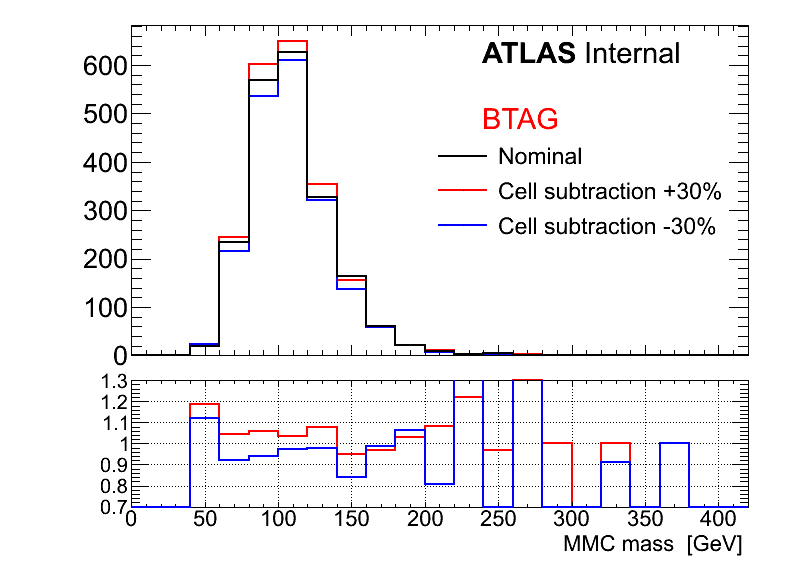
\includegraphics[width=0.49\textwidth]{figure/systematics/emb_sys_BtagFull_MFS.png}
	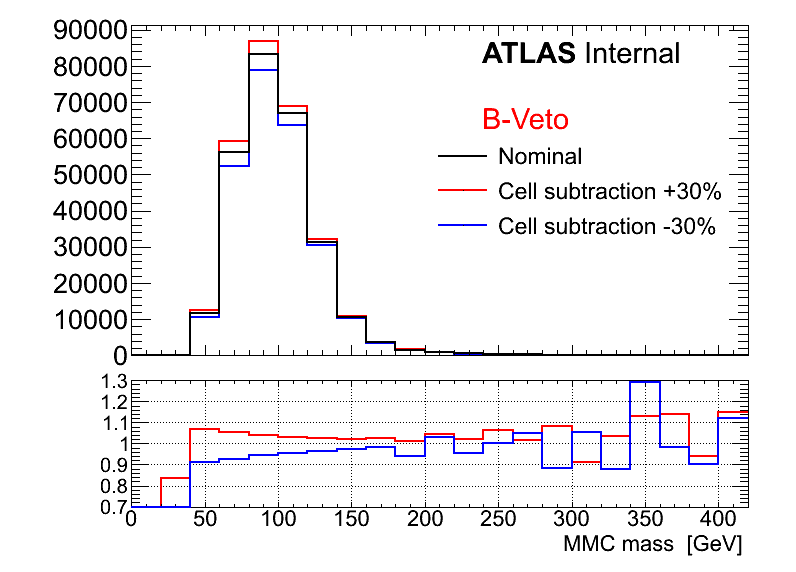
\includegraphics[width=0.49\textwidth]{figure/systematics/emb_sys_NoBtagFull_MFS.png}
	\end{center}
	\caption{Embedding MFS systematic uncertainty impact on $\mmc$.}
	\label{fig:EMBMFS}
\end{figure}

%\begin{figure}[htp]
%     \begin{center}
%
%        \subfigure[]{%
%            \label{fig:mvis}
%            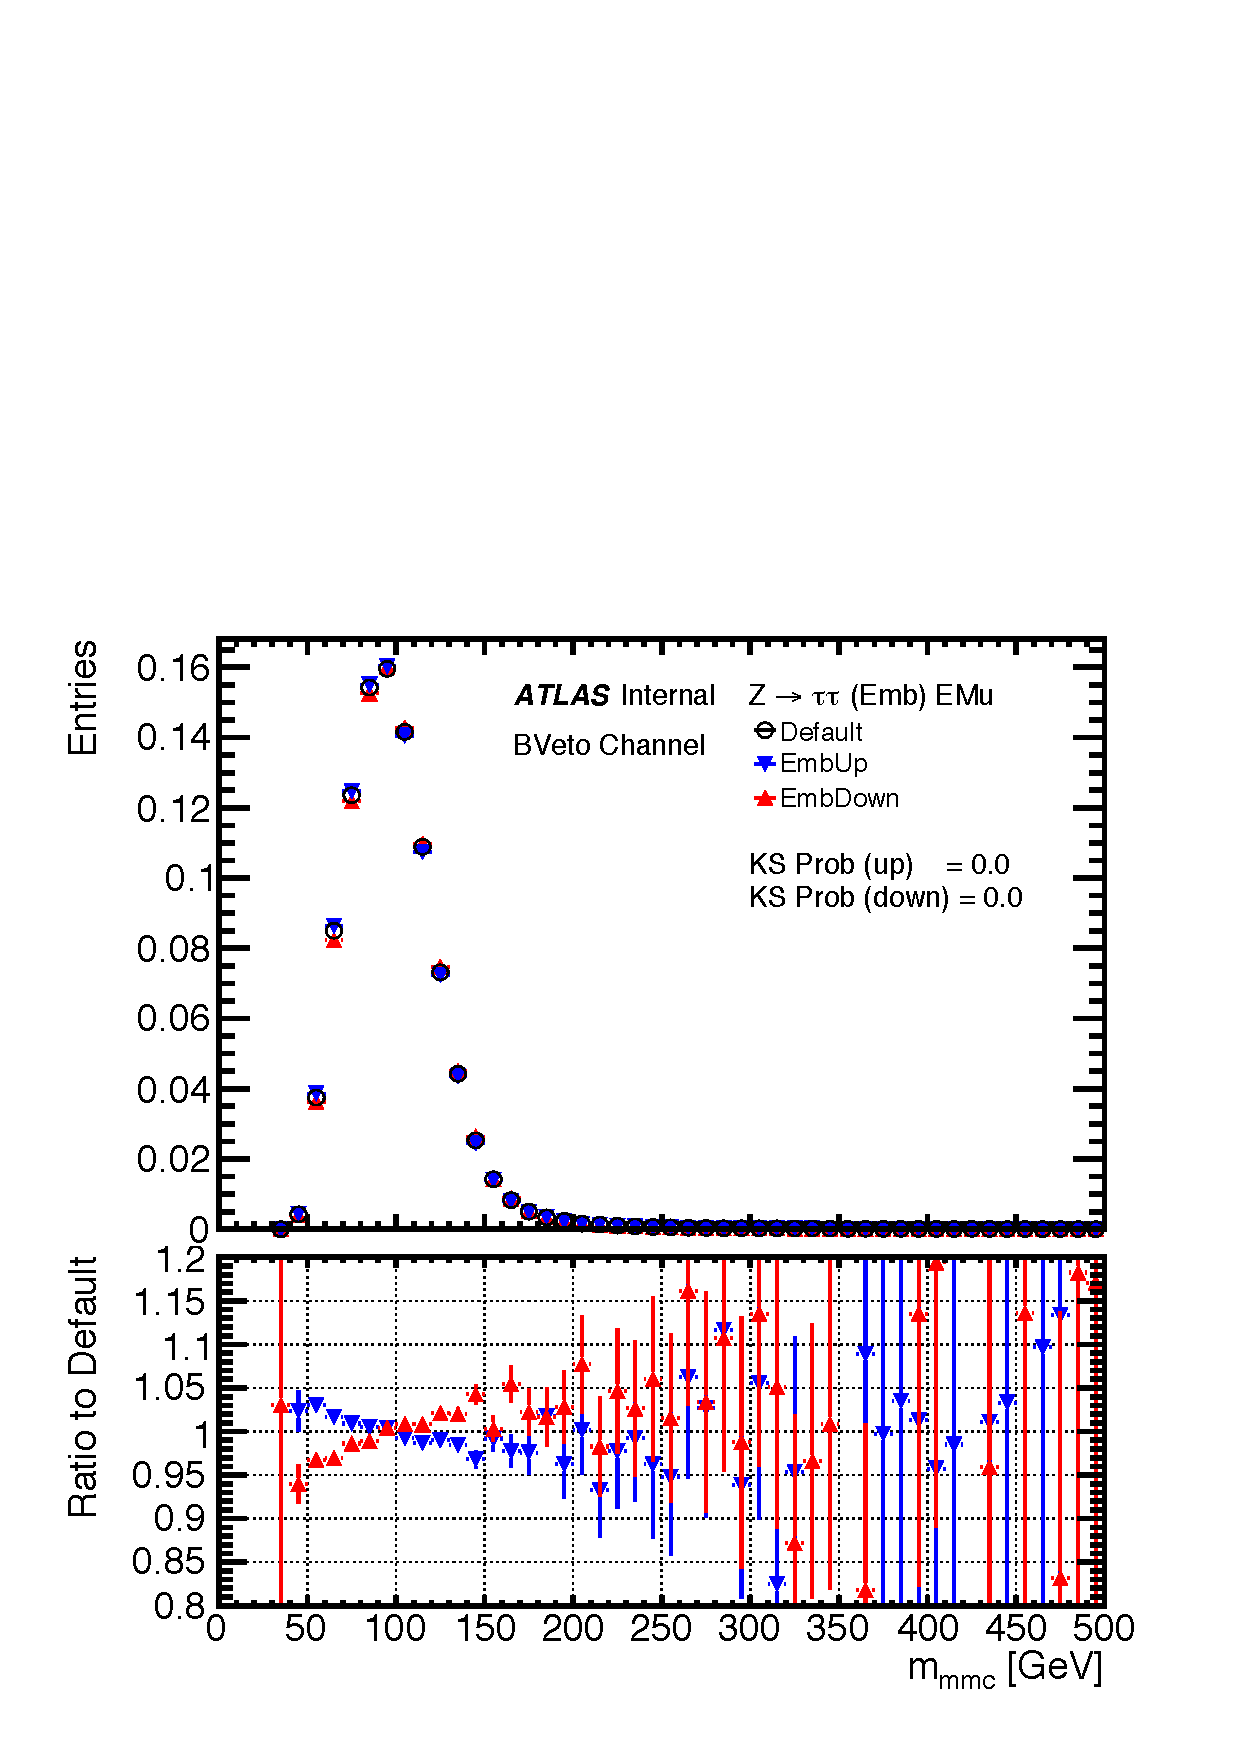
\includegraphics[width=0.45\textwidth]{figure/distributions/NP_Shape_EmbMFS_BVeto_mmc.pdf}
%	}
%	
%        \subfigure[]{%
%            \label{fig:mmc}
%            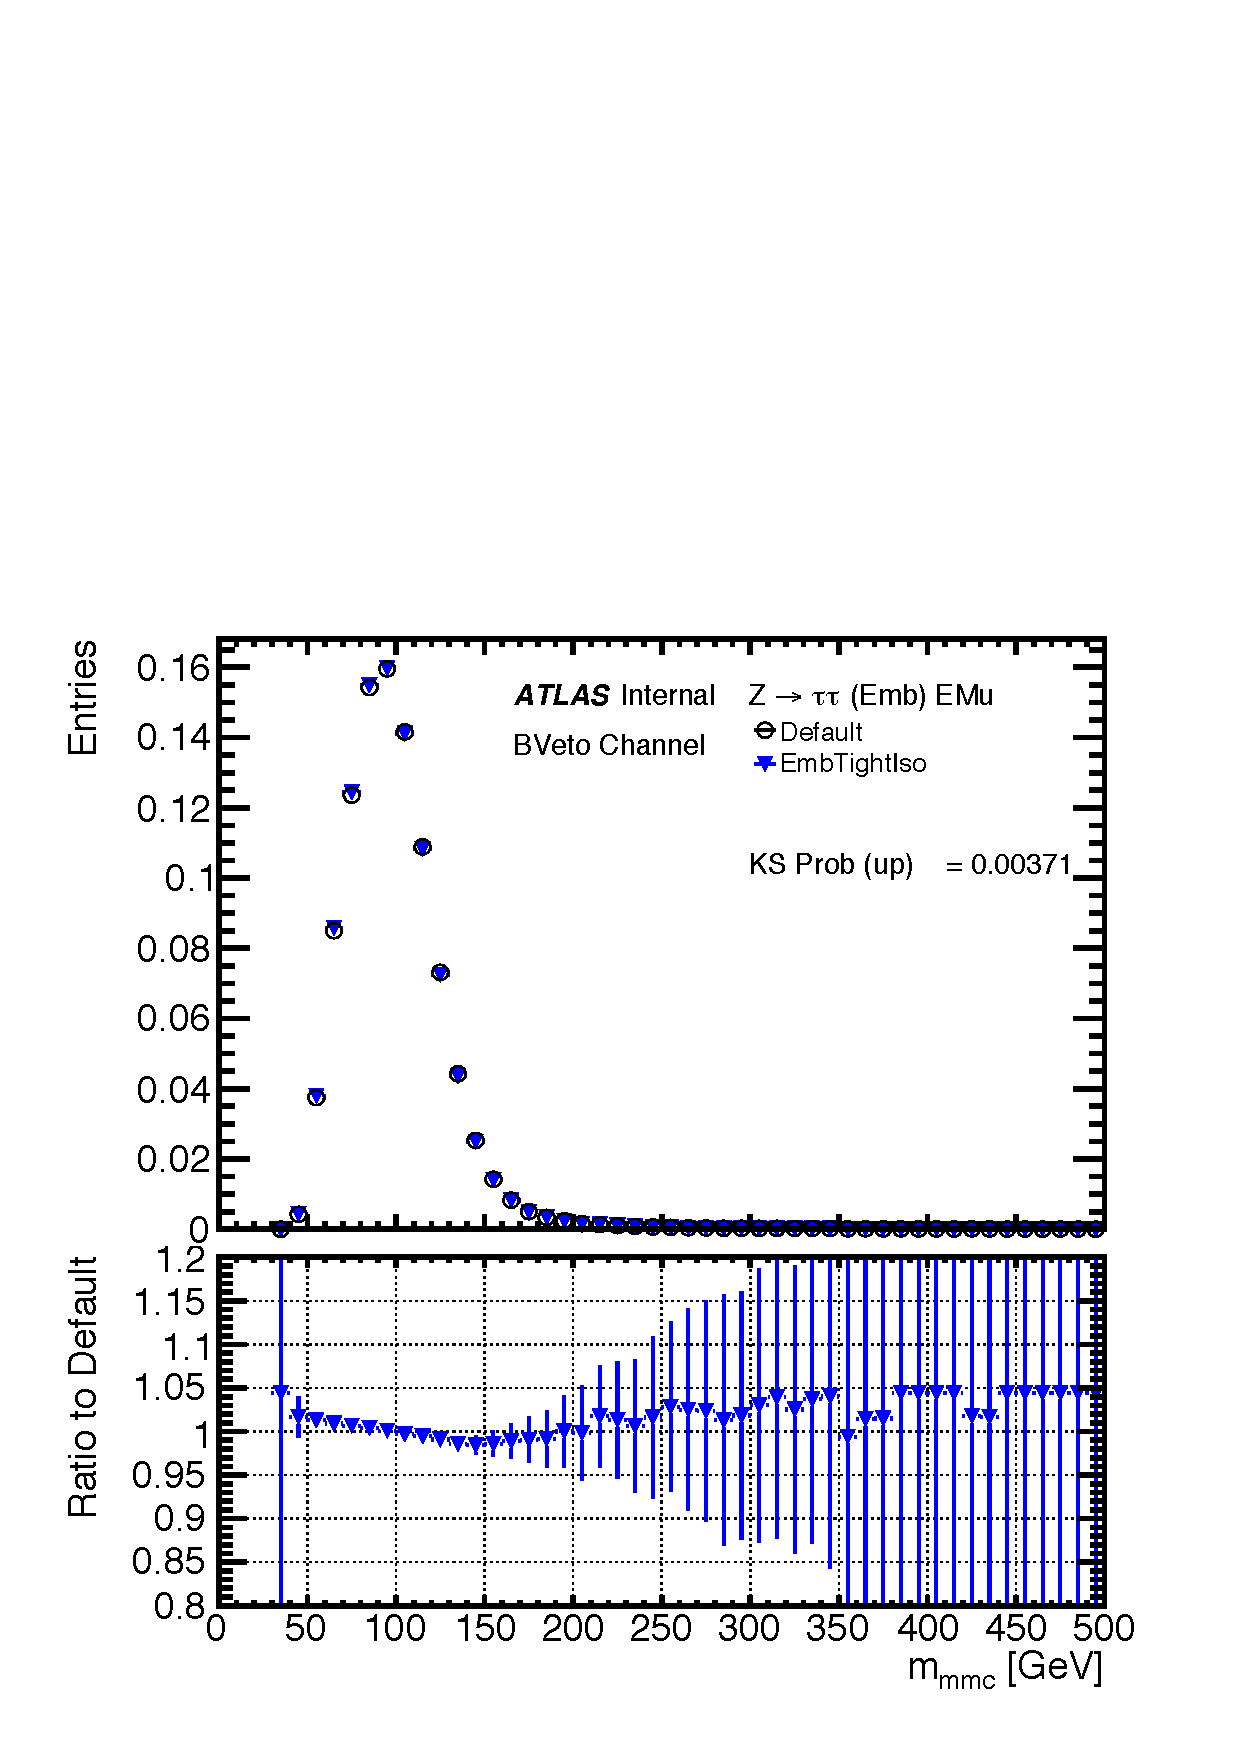
\includegraphics[width=0.45\textwidth]{figure/distributions/NP_Shape_EmbIso_BVeto_mmc.pdf}
%	}
%
%    \end{center}
%    \caption{Effect on the \mmc distribution of the embedding sample due to (a) the EMB\_MFS and (b) embedding isolation systematics. The plots are made after the full b-veto category selection.}
%   \label{fig:EmbeddingShapeNPs}
%\end{figure}

In the selection of the \Zmumu sample only a loose requirement on muon track isolation is required.
A different selection on the muon isolation may effect the selected sample by modifying the topology of the event, % since the requirement is indirectly acting also on the muon \PT, 
changing the non-\Zmumu contamination or the activity in the calorimeter. 
To estimate  the importance of these effects in our
embedding sample, the isolation selection on the muons in the original \Zmumu events is tightened to $\ptcone 40/ \PT<0.06$ and $\etcone 20/ \PT<0.04$, rather than the nominal selection of only $\ptcone 20/ \PT<0.2 $. 
A looser selection would have limited impact because of isolation requirements at trigger level.
The resulting uncertainty, referred to as EMB\_ISO, affects both the yield and the \mmc shape of the embedding samples, as shown in figure~\ref{fig:EmbeddingShapeNPs}. 

Finally, because the normalisation of the embedding sample is determined by the use of the ALPGEN sample, 
we also assign the relative cross section and luminosity uncertainties. In addition
all the detector-related systematic uncertainties relevant to the decay products of the simulated tau 
decay are propagated to the embedding sample.
 
\begin{figure}[tp]
	\begin{center}
	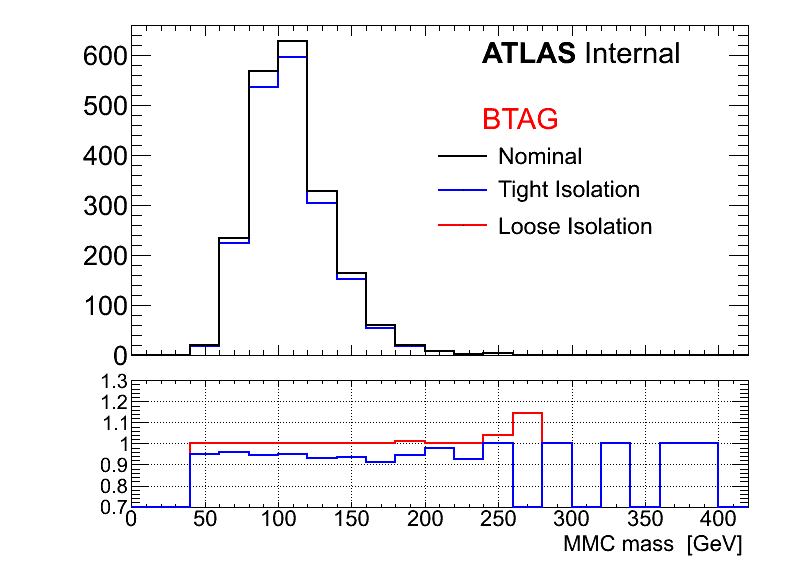
\includegraphics[width=0.49\textwidth]{figure/systematics/emb_sys_BtagFull_Iso.png}
	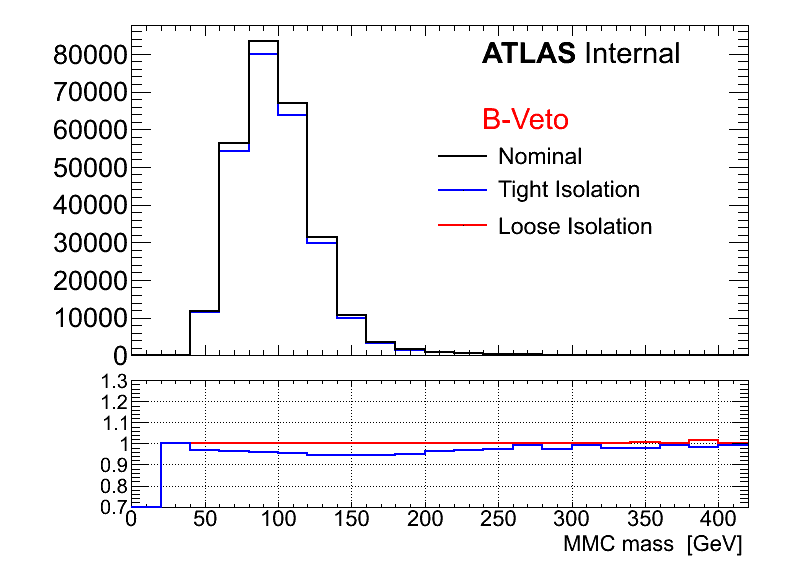
\includegraphics[width=0.49\textwidth]{figure/systematics/emb_sys_NoBtagFull_Iso.png}
	\end{center}
	\caption{Embedding Isolation systematic uncertainty impact $\mmc$.}
	\label{fig:EMBISO}
\end{figure}

\subsubsection{QCD Multi-Jet Systematics}

In this analysis the QCD multi-jet background is estimated via the ABCD method, as
described in Section~\ref{sec:qcd}. This technique relies strongly on
the assumption that the lepton isolation variables are independent from the
charge correlation between the two leptons. Systematic uncertainties
are assigned to take into account deviations from this assumption.
First we consider the correlation between \rqcd and the lepton isolation selections,
then we compare the result with an auxiliary method. 

Figure~\ref{fig:os_ss_ratio} shows the \rqcd factor, the ratio between the QCD 
yields in region C and D, as a function of the lepton isolation selections (red points).
%correlation is clearly visible. 
As described previously, the expectation from non-QCD backgrounds is subtracted from the data in regions C and D.
To estimate the uncertainty on the value of \rqcd  an additional transfer factor is defined as follows: $R_{QCD}^{iso}  = \hat{A} / \hat{B}$,
where  $\hat{A}$ and $\hat{B}$  are semi-isolated OS and SS regions defined with the lepton isolation larger than the standard requirement, 
but less than a sliding cut. Once more, the non-QCD contributions are subtracted from the data yields.
%$R_{QCD}^{iso}$ is an attempt to calculate a best estimate for the QCD transfer factor between isolated regions,
%which is in definitive the goal of the ABCD method. 
The regions $\hat{A}$ and $\hat{B}$ are chosen to be semi-isolated 
due to the high contamination of non-QCD background and possible signal in region A and B. 
Figure~\ref{fig:os_ss_ratio} shows $R_{QCD}^{iso}$ as a function of the lepton isolation selections (black points).
The difference between \rqcd and $R_{QCD}^{iso} $ in the vicinity of the standard cut value is then assigned as a systematic uncertainty on \rqcd. Using the point where the cuts on the lepton isolation are twice their standard values, a systematic uncertainty of 15\% is found.
The plot in Figure~\ref{fig:os_ss_ratio} is made at preselection level, similar plots using the full selection
for the two categories are in Appendix~\ref{appendix:qcd_additional}.

%for the definition of lepton isolations used in this analysis, the ratio is calculated in regions where the isolation requirements are reversed. Due to a high contamination of signal and non-QCD backgrounds, "semi-isolated" OS and SS regions are additionally defined, where the lepton isolation is larger than the standard requirement, but less than a sliding cut. These regions are labelled $\hat{A}$ and $\hat{B}$  for the semi-isolated OS and SS regions, respectively, and hence we can define $R_{QCD}^{iso}  = \hat{A} / \hat{B}$. The difference between \rqcd and $R_{QCD}^{iso} $ in the vicinity of our standard cut value is then assigned as a systematic uncertainty on \rqcd. Using the point where the cuts on the lepton isolation are twice their standard values, ie. the $x=100\%$ point on the graph, a systematic uncertainty of 15\% is found.

%An additional method considers calculating $\rqcd^{AB}$ as the ratio between the estimated QCD contributions in region A and B.
%These regions, however, suffers of large contribution of non-QCD background and possible signal contamination, 
%this method is then only used as a cross check. Table~\ref{table:MCsub} shows a comparison between \rqcd and  $\rqcd^{AB}$
%for the two category at an early stage of the cutflow where signal contamination is negligible, agreement is seen within statistical uncertainties.

An additional method, used as a crosscheck, considers calculating \rqcd as the ratio between the estimated QCD contributions in region A 
and B. Here the non-QCD contributions are once more subtracted from data. However the large contribution of this non-QCD background, 
along with lack of statistics and possible signal contamination, lead to this only being used as a cross check. Table~\ref{table:MCsub} shows 
a comparison between \rqcd and $\rqcd^{AB}$ for the two categories at the preselection stage of the cutflow, where signal contamination is negligible. 
Agreement is seen between \rqcd values in the two regions, within statistical uncertainties. 

%\footnote{This effect is maybe due to the use of a \PT dependent isolation variable that effects the quark-gluon fraction.}.
%Expectation for non-QCD backgrounds are subtracted as usual. 
%This effect however doesn't tell anything on the uncertainty of our
%measure of \rqcd, we want to measure instead what is the discrepancy (for each
%choosen isolation cut value) between \rqcd and the same factor calculated 
%flipping isolation requirements, i.e. using the isolated regions A and B, we call this factor $R_{QCD}^{iso}$. 
%Due to the high contamination of non-QCD backgrounds and signal in these regions we then define:
%OS and SS isolated regions $\hat{A}$ and $\hat{B}$ in wich the leptons isolation
%should be greather than the standard value but less of predefined quantity on the x axis 
%of the graph (black curve). In definitive we have $R_{QCD}^{iso}  = \hat{A} / \hat{B}$.
%We then assign as a systematics uncertainty the difference between the two curves (red and black) in the vicinity of our
%standard cut value (we use the point where the cut value is doubled, 100\% in the graph because 
%of statistical fluctuation), our estimate of the systematics uncertainty on \rqcd is then 15\%.
%The plot in Figure~\ref{fig:os_ss_ratio} is made at preselection level, similar plots using the full selection
%for the two categories are in Appendix~\ref{appendix:qcd_additional}.

%An additional method used as a crosscheck relies on the definition of "real-$\rqcd$" as the pure ratio between region A and B (non-QCD background
%estimate is subtracted from data in each regions), this would be the exact factor 
%that allows you to extrapolate yield from region B to SR, however it suffer of contamination by non-QCD backgrounds
%and lack of statistics.
%Table~\ref{table:MCsub} shows comparison between \rqcd and real-\rqcd
%for the two category at an early stage of the cutflow where signal contamination is negligible.
%Discrepancies are within statistical uncertainty and underline that an assignment of a  15\%
%uncertainty to the \rqcd factor is conservative.

 %How this is actually implemented in limits machinery
The actual implementation in the limit framework of the ABCD method follows that suggested in~\cite{ABCD}.
Here three free parameters are fitted: number of multi-jet events in region B, $N_{B}^{QCD}$, factor that extrapolates from SS region to OS regions, \rqcd, and the factor that 
extrapolates from isolated to anti-isolated regions $R_{BD}$. Neglecting signal contributions, the following 
equations can be written for the event yield of the B,C and D control regions:
%$$N_{B} = N_{B}^{BKG} + N_{B}^{QCD} $$ 
%$$N_{C} = N_{C}^{BKG} +  N_{B}^{QCD} \times \rqcd \times R_{BD} $$
%$$N_{D} =  N_{D}^{BKG} + N_{B}^{QCD} \times  R_{BD} $$
\begin{itemize}
\item[] $N_{B} = N_{B}^{BKG} + N_{B}^{QCD}$
\item[] $N_{C} = N_{C}^{BKG} +  N_{B}^{QCD} \times \rqcd \times R_{BD} $
\item[] $N_{D} =  N_{D}^{BKG} + N_{B}^{QCD} \times  R_{BD} $
\end{itemize}
where $N^{BKG}$ represent the prediction of  non-QCD background in the relative regions.
The estimate of multi-jet event yield in SR will be then $ N_{B}^{QCD} \times \rqcd $. This method is 
particularly powerful because in the best fit of \rqcd the statistical 
and systematics uncertainty for non-QCD backgrounds and data will be considered.


\begin{table} [tp]
	\begin{center}
	\begin{tabular}{l  c c c }
%%%%%%%%%%%%%%%%%%%%%%%%%%%%%%%%%%%%%%%%%%%%%%%%%%%%%%
\hline 
\hline
Selection  		&  \rqcd  			&  $\rqcd^{AB}$  		&  $R_{QCD}^{iso}$ \\ 
\hline
Preselection 		&   1.929 $\pm$     0.004	&	2.12 $\pm$ 0.17		&	2.22 $\pm$ 0.16	\\
B-veto			&  1.965   $\pm$   0.005    	& 2.10   $\pm$	0.16 		&	2.22 $\pm$ 0.16	\\
B-tag			&  1.78    $\pm$   0.02 	& 1.9   $\pm$	0.9 		&	2.0  $\pm$ 0.8	\\
\hline
\hline
%%%%%%%%%%%%%%%%%%%%%%%%%%%%%%%%%%%%%%%%%%%%%%%%%%%%%%
	\end{tabular}
	  \caption{Comparison between \rqcd, $\rqcd^{AB}$ and $R_{QCD}^{iso}$ for early stage in the cutflow, only b-tag and b-veto
	requirement are applied after preselections. Reported is statistical uncertainty only.}
	\label{table:MCsub}
	\end{center}
\end{table}


\begin{figure}[tp]
	\begin{center}
	\includegraphics[page=5,width=0.9\textwidth]{figure/QCD/qcd_plot.pdf}
	\end{center}
	\caption{OS/SS ratio as a function of lepton isolation variable selections. The selections are varied as a percentage relative to
	the standard lepton isolation cut values (0~in the plot). 
	%As an example the point at 100\% in the plot corresponds
	%to $\rqcd$ evaluated by increasing the isolation requirement by 100\% respect to the standard cut value.
	The red points show the anti-isolated scale factor $\rqcd$, i.e. the ratio between regions C and D.
	 The black points show the isolated SF, which is defined as the ratio between region $\hat{A}$ and $\hat{B}$, 
	 where the leptons have isolation values larger than the nominal value but smaller
	 than the sliding cut on X axis.
%	 taking the same example point at 100\%, than the double of the standard cut value.
	 }
	\label{fig:os_ss_ratio}
\end{figure}

The difference in \mmc shape observed between the OS and SS anti-isolated regions (C and D) is shown in Figure~\ref{fig:qcd_shape_unc}.
This effect is within the  uncertainty on \rqcd of the ABCD method, hence no correction factor is applied to the mass shape. We assume, however, that there could be the same 
shape difference in the isolated regions. Hence a shape uncertainty is assigned in the limit machinery to region B with this deviation. Further 
shape uncertainties due to non-QCD background subtraction are found to be negligible. The uncertainty due to the use of an isolation 
requirement at trigger level is discussed in Appendix~\ref{appendix:qcd} and is found to be negligible.


\begin{figure}[tp]
	\begin{center}
	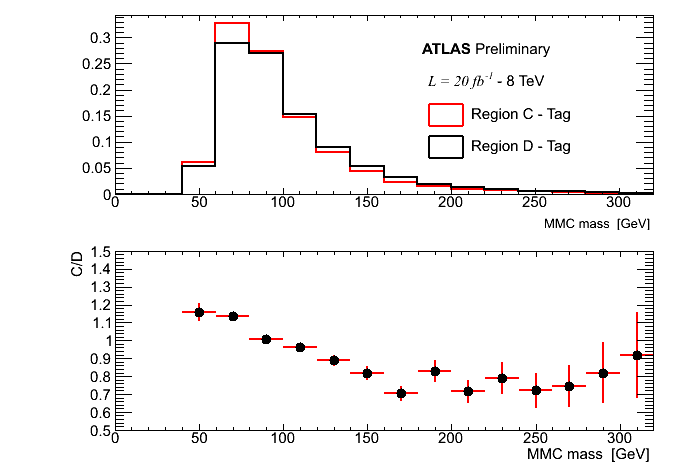
\includegraphics[width=0.65\textwidth]{figure/QCD/shape_tag.png}
	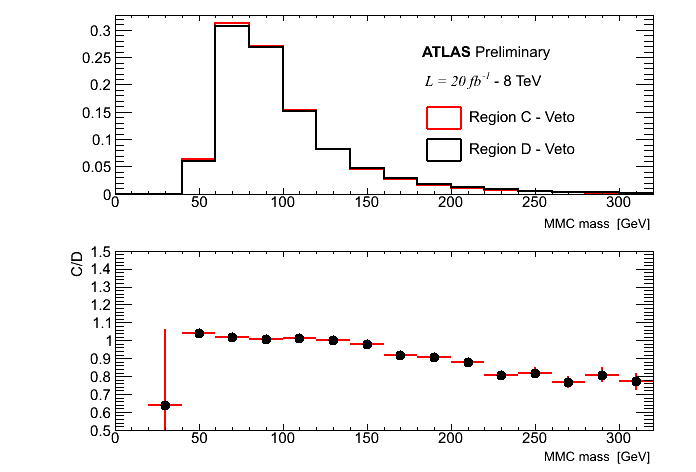
\includegraphics[width=0.65\textwidth]{figure/QCD/shape_veto.png}
	\end{center}
	\caption{Shape differences for the b-tag and b-veto categories between the ABCD regions C and D.}
	\label{fig:qcd_shape_unc}
\end{figure}

\subsection{Theoretical Uncertainties}
\label{sec:sys_theory}

\subsubsection{Simulated Cross-Section Uncertainties}
Uncertainties on the cross-sections that have been used to normalise
simulation samples to data are reported in
Table~\ref{table:sys_xsec}. These
uncertainties include contributions due to parton distribution
functions (PDFs), the choice of the value of strong coupling constant,
and the renormalisation and factorisation scales.  Furthermore the
uncertainties on signal cross-section depends on $\tan\beta$, the
Higgs boson type ($A$/$h$/$H$) and mass.

\begin{table} [t]
\centering
\begin{tabular}{c c c }
\hline
\hline
Generator & Process & Uncertainty \\ [0.5ex]
\hline
ALPGEN & $Z \rightarrow \tau\tau / ee /\mu\mu$ & $\pm 5\%$ \\
POWHEG & \ttbar					& $\pm 5.5\%$\\
ALPGEN & $W  \rightarrow \tau\nu / e\nu /\mu\nu$&  $\pm  5\%$ \\
AcerMC & single top & $\pm 13 \%$ \\
HERWIG & dibosons & $\pm 6 \%$ \\
SHERPA & $bbA$/$h$/$H$  ($m_{A} \ge 120$~GeV)     & $-(<20)$\%,  $+(<9)$ \%\\
SHERPA & $bbA$/$h$/$H$  ($m_{A} =   110$~GeV)     & $-(<25)$\%,  $+(<9)$ \%\\
SHERPA & $bbA$/$h$/$H$  ($m_{A} =   100$~GeV)     & $-(<28)$\%,  $+(<9)$ \%\\
SHERPA & $bbA$/$h$/$H$  ($m_{A} =    90$~GeV)     & $-(<30)$\%,  $+(<9)$ \%\\
POWHEG & $ggA$/$h$/$H$  ($m_{A} \le 300$~GeV)     & $<$ 15\%\\  [0.5ex]
\hline \hline 
\end{tabular}
\caption{Cross-section uncertainties for background and signal samples.The reported signal samples are all for $\tan\beta = 20$.}
\label{table:sys_xsec}
\end{table}

\subsubsection{Acceptance Systematics}

The effect of systematic uncertainties due to various MC tuning
parameters, underlying event and
lepton kinematic description is considered.
Since the effect on the invariant mass distribution of the di-tau system from these systematic
uncertainties is negligible (as an example see
Figure~\ref{fig:theory_mass} ), only the variation in
acceptance is considered as systematic uncertainty.

The acceptance uncertainties for the ALPGEN Z MC, used for the normalisation of the embedded sample, 
are estimated at lepton preselection to be 4\% \cite{2010SMLLSupportNote}.
%\footnote{A bit old result, to be reviewed. Depends also on the
%embedding choice}
Since additional selections are applied directly to the embedded sample, 
no further acceptance uncertainties is considered. Acceptance systematics on
$t\bar{t}$ simulated events are still to be determined. %\textcolor{red}{still to be added}.
%evaluated
%\footnote{also here is not totally clear yet} 
%by the difference between MC@NLO and POWHEG in
%the data-driven background estimate. 
%For other, single and dibosons
%production as well as single top production a 2\% uncertainty is
%assumed.
The acceptance uncertainties on diboson and single top production are assumed to be 2\%.
%\footnote{preliminary, this is following LEP-Had note, we
%  should cite some previous result here.}.

Uncertainties on signal acceptance have been estimated
by producing samples with varied MC generator parameters and evaluating, at
truth-level, the effect of analysis selections on leptons, taus and
jets. This truth-level study is implemented within the Rivet framework
\cite{RIVET}, where additionally b-tagging is performed by identifying b-quarks and applying
a weighting according to the estimated ATLAS b-tagging
efficiencies \cite{BtaggingScaleFactors}. The variation of the acceptance
with respect to the nominal MC tune has also been considered as
a source of systematic uncertainty.
%INCOMPLETE---missing energy??? I don't remember... to ask Lorentz...

The acceptance uncertainties of the two signal production modes are
evaluated separately because of the use of different generators for each. For
b-quark associated production, generated with SHERPA,
the CKKW matching parameter $Q_{cut}$ has been varied from its default
of $\sqrt{20 ~ GeV/E_{CMS}}$ to values of $\sqrt{15 ~ GeV/E_{CMS}}$
and $\sqrt{30 ~ GeV/E_{CMS}}$. The factorisation scale was varied up
and down by a factor of two and the renormalisation scale by a factor of
10\%. Uncertainties due to the PDFs were determined by taking the RMS
of the acceptance of the 52 error sets of the CT10 PDF set.  These
effects are summarised in Table~\ref{table:sys_bba}. For a total
uncertainty, all effects are summed in quadrature giving a total
uncertainties that varies from 4\% to 30\% depending on $\mA$ and on the
analysis category.  For gluon fusion production, generated with POWHEG
and Pythia 8, the initial and final state
radiation uncertainties were varied up and down, and the
renormalisation and factorisation scales were varied simultaneously
(the renormalisation scale by 10\% and the factorisation scale by factor 2\%).
PDFs uncertainties were handled in the same way as for the $b$-quark
associated production.  These variations are summarised in Table
\ref{table:sys_gga}.  The uncertainties shown in Tables
\ref{table:sys_bba} and \ref{table:sys_gga} are based on samples with
$m_{A} = 120 \text{ GeV}$.  Results for the mass points 90, 200
and 300 GeV are shown in Appendix \ref{appendix:additional} of this note.
 

\begin{figure}[tdp]
\begin{center}
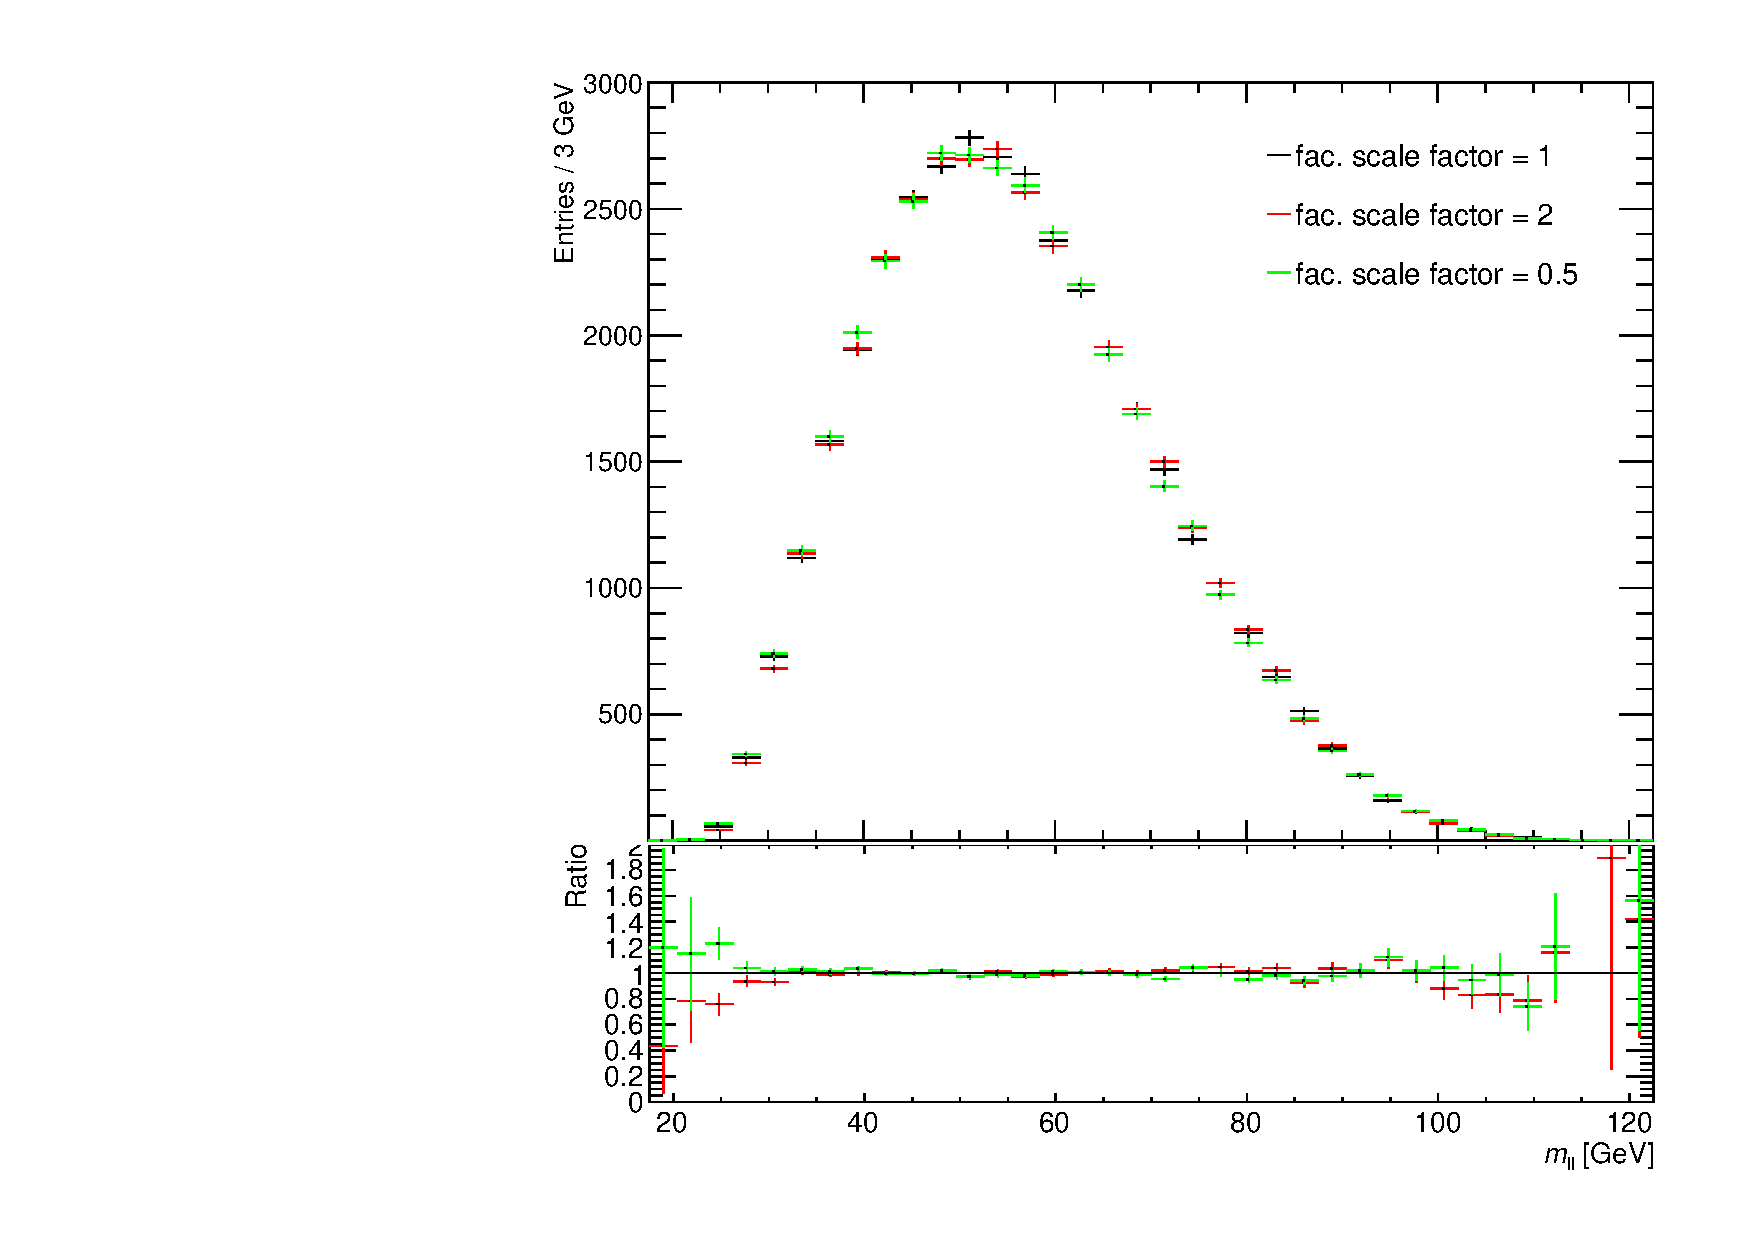
\includegraphics[width=8cm]{figure/facs_mll_bveto}
\end{center}
\caption{ Comparison of the visible mass of tau decay products after factorisation scale variation for the b-veto category on a gluon fusion signal sample.}
\label{fig:theory_mass}
\end{figure}


\begin{table}[tdp]
  \begin{center}
   \label{table:sys_bba}
   \begin{tabular}{lccccc}
\hline \hline
 Event yields       & b-tag deviation [\%]  & b-veto deviation [\%] \\
\hline
CKKW down &    $ -3.1 \pm 0.9 $ &      $ 0.4 \pm 0.4 $ \\
CKKW up &     $ -8.3 \pm 0.9 $ &      $ 2.9 \pm 0.4 $ \\
Fac. scale down &    $ 15.5 \pm 1.0 $ &   $ -4.2 \pm 0.4 $ \\
Fac. scale up &     $ -19.8 \pm 0.8 $ &    $ 5.6 \pm 0.4 $ \\
Ren. scale down &      $ 0.4 \pm 0.9 $ &     $ -0.3 \pm 0.4 $ \\
Ren. scale up &     $ 0.8 \pm 0.9 $ &      $ 0.5 \pm 0.4 $ \\
PDF &     $\pm 0.1 $ 		& $\pm 0.2 $ \\
\hline
Total  (up) &     $ 13.5 \pm 1.6$ &                    $ 6.3 \pm 0.8$ \\
Total  (down) &     $ -21.7 \pm 1.5$ &                    $ -4.2 \pm 0.6$ \\ 
\hline \hline
	\end{tabular}
   \caption{Signal acceptances for several systematic deviations of the theory parameters contributing to the b-quark associated production of Higgs bosons. The different variations are added in quadrature to a total uncertainty on the signal acceptance in the b-tag and b-veto channels.}
  \end{center}
\end{table}


\begin{table}[tdp]
  \begin{center}
   \label{table:sys_gga}
    \begin{tabular}{lccccc}
    \hline \hline
 Event yields      &   b-tag deviation [\%] &   b-veto deviation [\%] \\
\hline
ISR up & $ 20.3 \pm 8.1 $ 		& $ -1.2 \pm 0.6 $ \\
ISR down & $ 3.6 \pm 7.2 $ 		& $ 0.4 \pm 0.6 $ \\
FSR up & $ 16.6 \pm 7.8 $ 		& $ -0.2 \pm 0.6 $ \\
FSR down & $ -3.6 \pm 6.8 $	 	& $ -0.7 \pm 0.6 $ \\
Ren./Fac. scales up & $ 9.4 \pm 7.5 $ 	& $ 0.0 \pm 0.6 $ \\
Ren./Fac. scales down & $ 2.5 \pm 7.1 $ & $ -0.5 \pm 0.6$ \\
PDF &     $\pm 0.0 $ &$\pm  0.1 $ \\
\hline
Total (up) &    $ 28.2 \pm 16.9 $ &     $ 0.4 \pm 0.6$ \\
Total (down) &    $ -3.6 \pm 6.8 $ &     $ -1.5 \pm 1.2$ \\ 
\hline \hline
	\end{tabular}
   \caption{Signal acceptances for several systematic deviations of the theory parameters contributing to the Higgs boson production through gluon fusion. The different variations are added in quadrature to a total uncertainty on the signal acceptance in the b-tag and b-veto channels.}
  \end{center}
\end{table}



